\documentclass[10pt,a4paper]{article}
\usepackage[margin=21mm,headheight=14pt]{geometry}
\usepackage{fontspec,graphicx,float,amsmath,xcolor,titlesec,needspace}
\usepackage{hyperref}
\usepackage{fancyhdr}
\usepackage[numbers]{natbib}
\setmainfont[Path=../assets/fonts/,BoldFont=Estedad-Bold.ttf,ItalicFont=Estedad-Medium.ttf,Script=Arabic,Language=Persian]{Estedad-Medium.ttf}
\newfontfamily\latinfont[Path=../assets/fonts/,BoldFont=DejaVuSans-Bold.ttf]{DejaVuSans.ttf}
\TeXXeTstate=1
\newcommand{\rtl}[1]{\beginR #1\endR}
\newcommand{\lr}[1]{\beginL{\latinfont #1}\endL}
\newcommand{\rp}[1]{\par\begingroup\rightskip=0pt\leftskip=0pt plus 1fil\parfillskip=0pt\noindent\beginR #1\endR\par\endgroup}
\renewcommand{\figurename}{\rtl{شکل}}
\renewcommand{\tablename}{\rtl{جدول}}
\renewcommand{\refname}{\rtl{مراجع}}
\hypersetup{hidelinks,pdftitle={SDR Laboratory Report},pdfauthor={SDR Lab Team}}
\pdfstringdefDisableCommands{\def\rtl#1{#1}\def\lr#1{#1}}
\setlength{\parindent}{0pt}\setlength{\parskip}{7pt}
\linespread{1.32}
\titleformat{\section}{\large\bfseries\raggedleft}{\thesection}{1em}{}
\pagestyle{fancy}\fancyhf{}\fancyhead[L]{\small\lr{SDR LAB}}\fancyfoot[C]{\thepage}
\renewcommand{\labelitemi}{\lr{-}}
\begin{document}
\fancyhead[R]{\small\rtl{آزمایش ۱ | گزارش پس از جلسه}}
\begin{titlepage}\begin{center}\vspace*{12mm}
{\color{teal}\Large\lr{LAB01 / POST}}\\[12mm]
{\LARGE\bfseries\rtl{گزارش آزمایش ۱: پایش طیف}}\\[9mm]
\rtl{گروه آزمایشگاه \lr{SDR}}\\[4mm]
\rtl{دکتر سید محمد کرباسی}\\[4mm]
\rtl{نیمسال اول ۱۴۰۵-۱۴۰۶}\\[4mm]
\vspace{10mm}
\rtl{عضو ۱؛ نام و نام خانوادگی: سروش مومنی}\\[5mm]
\rtl{شمارهٔ دانشجویی: \lr{402102538}}\\[9mm]
\rtl{عضو ۲؛ نام و نام خانوادگی: مهدی قلمی نوبر}\\[5mm]
\rtl{شمارهٔ دانشجویی: \lr{402102284}}\\[9mm]
\rtl{تاریخ جلسه: ۲۰۲۶/۱۱/۰۴ - طبق نام ثبت‌های کنسول}\\[4mm]
\rtl{تحویل: تاریخ ثبت تحویل هنوز اعلام نشده}\\[8mm]
\end{center}
\begin{quote}\rp{وضعیت این نسخه: گزارش تصویری آمادهٔ بازبینی؛ تحلیل عددی دادهٔ خام هنوز انجام نشده است. این نسخه تحویل نهایی کامل دستور کار محسوب نمی‌شود.}

\end{quote}
\end{titlepage}
\Needspace{6\baselineskip}
\section{\rtl{چکیده و حدود اعتبار}}
\rp{در این آزمایش، ارتباط شبکه‌ای با رادیوی نرم‌افزاری برقرار شد، تنظیمات واقعی گیرنده بازخوانی شد، نگاشت فرکانس با تن مختلط در اتصال حلقه بررسی شد و طیف باند ریموت و دو جهت ارتباط سلولی مشاهده شد. دو بلوک پهن در حدود ۹۴۲ تا ۹۵۲ مگاهرتز، سیگنال گذرای نزدیک ۴۳۳٫۹۲ مگاهرتز و افزایش فعالیت فراسو پس از تماس، مهم‌ترین مشاهده‌های تصاویرند.}

\rp{این نسخه گزارش مستندات تصویری است. ۳۷ تصویر اصلی بررسی شده‌اند؛ فایل خام \lr{IQ} هنوز تحویل نشده است. اعداد تقریبی طیف در متن، خوانش محور تصویرند و اندازه‌گیری نهایی از نمونه‌ها محسوب نمی‌شوند. \lr{Welch}، پهنای اشغالی ۹۹٪، مدت و دورهٔ برست، \lr{ppm} و تطبیق پنج سیگنال با فایل خام پس از دریافت \lr{IQ} تکمیل می‌شوند. از ساختن عدد یا نمودار تجربی جایگزین دادهٔ خام خودداری شده است.}

\rp{تاریخ ۲۰۲۶/۱۱/۰۴ از نام فایل‌های کنسول برداشت شده است؛ ساعت و تاریخ رایانه نیازمند تأیید گروه است. پیش‌گزارش موجود فقط فایل‌های فلوگراف و ضبط‌کننده را دربر دارد؛ جدول عددی پیش‌بینی و احتمال رهگیری در آن ارائه نشده است.}

\Needspace{6\baselineskip}
\section{\rtl{۱. دستگاه، اتصال و تنظیمات واقعی}}
\rp{برخلاف نام عمومی \lr{ADALM-Pluto} در دستور کار، خروجی خود دستگاه در \lr{command\_properties.png} مدل \lr{PUZHI PZSDR P201PRO} و تراشهٔ \lr{ad9361} را گزارش می‌کند. بنابراین مشخصات \lr{AD9363} در جدول دستور کار، به‌ویژه دقت مرجع \lr{±}۲۵ \lr{ppm}، مشخصهٔ تأییدشدهٔ این دستگاه نیست. رابط مورد استفاده \lr{libiio} و آدرس \lr{ip:192.168.1.10} است.}

\rp{جدول \ref{tab:settings} اطلاعات این بخش را ثبت می‌کند.}
\begin{table}[H]\centering\small\renewcommand{\arraystretch}{1.25}
\begin{tabular}{|p{0.445\linewidth}|p{0.445\linewidth}|}\hline
\rtl{\textbf{مقدار ثبت‌شده}} & \rtl{\textbf{کمیت}} \\ \hline
\rtl{\lr{PUZHI PZSDR P201PRO / ad9361}} & \rtl{مدل / تراشه} \\ \hline
\rtl{\lr{3669-dirty}} & \rtl{\lr{Firmware}} \\ \hline
\rtl{[\lr{70000000 1 6000000000] Hz}؛ از ۷۰ مگاهرتز تا ۶ گیگاهرتز} & \rtl{بازهٔ \lr{RX LO}} \\ \hline
\rtl{۴ پاسخ از ۴ درخواست؛ صفر درصد اتلاف؛ زمان رفت‌وبرگشت ۱ تا ۲ \lr{ms}} & \rtl{آزمون \lr{ping}} \\ \hline
\rtl{\lr{945000000 Hz}} & \rtl{\lr{RX LO} واقعی} \\ \hline
\rtl{\lr{2600000 S/s}} & \rtl{نرخ واقعی} \\ \hline
\rtl{\lr{20000000 Hz}} & \rtl{پهنای فیلتر \lr{RF}} \\ \hline
\rtl{\lr{manual / 20 dB}} & \rtl{حالت و بهره} \\ \hline
\end{tabular}\caption{\rtl{مقادیر مستقیماً خوانده‌شده از کنسول}}\label{tab:settings}\end{table}
\rp{تصویر ثبت‌شده در شکل \ref{fig:1} آمده است.}
\begin{figure}[H]\centering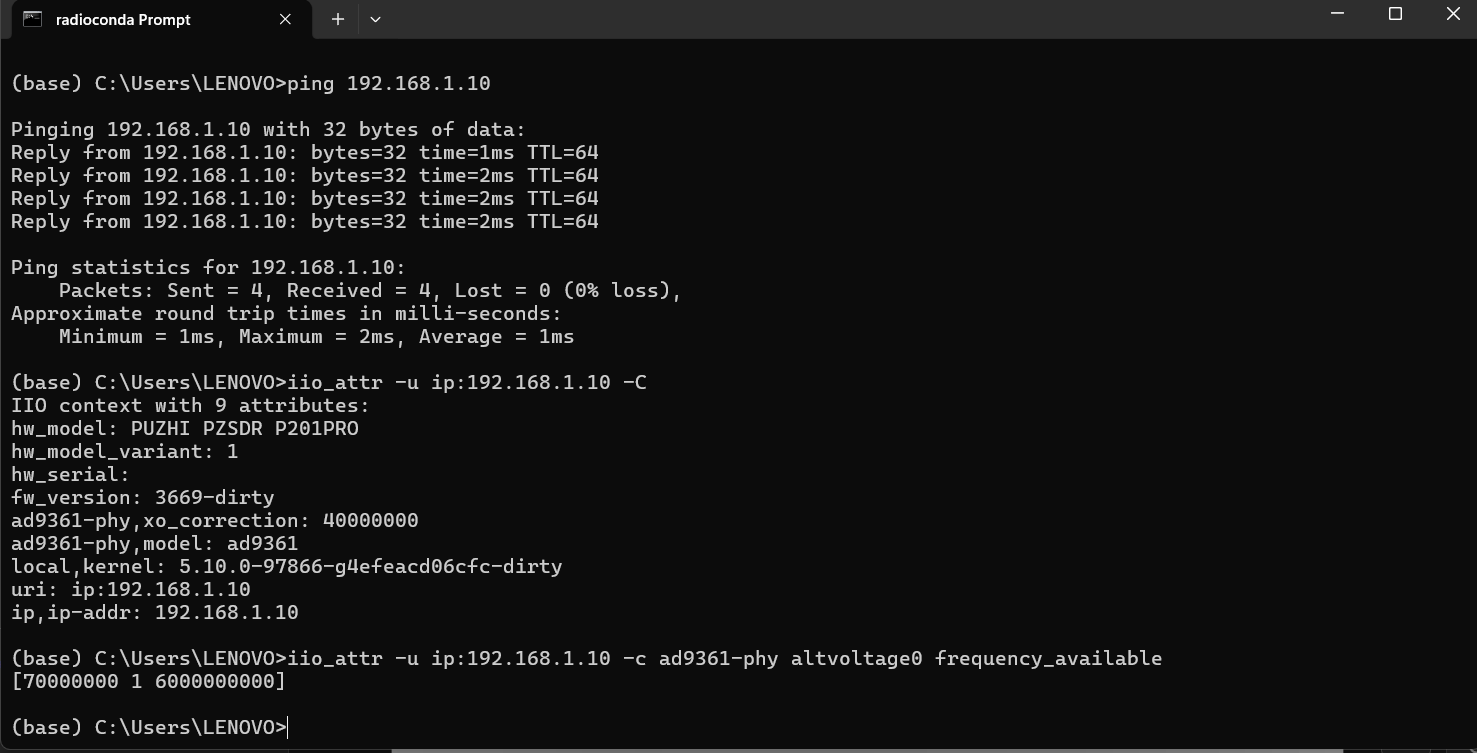
\includegraphics[width=0.96\linewidth,height=0.29\textheight,keepaspectratio]{../assets/images/lab01/command_properties.png}\caption{\rtl{شناسایی سخت‌افزار، پاسخ شبکه و بازهٔ واقعی \lr{LO}؛ مرجع مشخصات دستگاه همین خروجی است.}}\label{fig:1}\end{figure}
\rp{تصویر ثبت‌شده در شکل \ref{fig:2} آمده است.}
\begin{figure}[H]\centering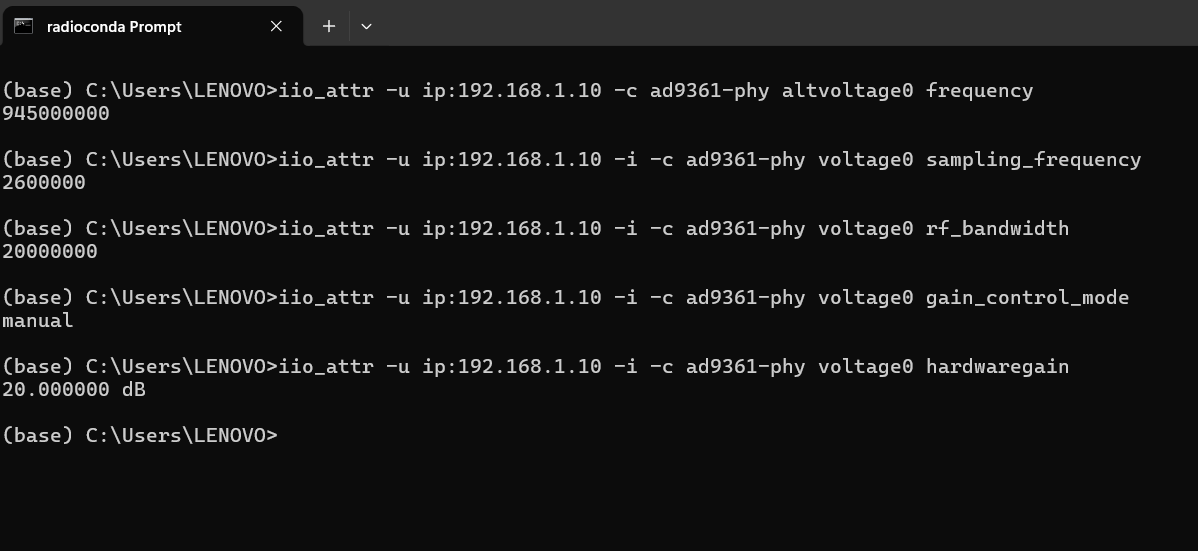
\includegraphics[width=0.96\linewidth,height=0.29\textheight,keepaspectratio]{../assets/images/lab01/real_values.png}\caption{\rtl{بازخوانی پنج پارامتر واقعی گیرنده در زمان اجرا.}}\label{fig:2}\end{figure}
\rp{در دریافت هوایی طبق دستور کار آنتن روی \lr{RX1} و فرستنده بدون آنتن است. آزمون حلقه باید با کابل \lr{TX1} به \lr{RX1}، بهرهٔ \lr{RX} حداکثر ۱۰ \lr{dB} و تضعیف \lr{TX} حداقل ۴۰ \lr{dB} انجام شود. اتصال فیزیکی و تضعیف واقعی از این تصاویر به‌تنهایی قابل تأیید نیست. فلوگراف موجود سقف بهرهٔ حلقه را ۱۰ و کف تضعیف را ۴۰ \lr{dB} قرار داده است؛ مقدار اولیهٔ تضعیف در فایل ۶۹ \lr{dB} است.}

\rp{۲۰ \lr{dB} یک بهرهٔ ثبت‌شده است، نه بیشترین بهرهٔ بهینهٔ اثبات‌شده. نام یکی از تصاویر به تغییر ۲۴ به صفر اشاره دارد، ولی یک پیمایش مستند با گام‌های ۵ \lr{dB} و دامنهٔ زمانی هر مرحله موجود نیست. در نمای پهن دامنهٔ \lr{I} و \lr{Q} حدود چند دهم یا کمتر از مقیاس کامل دیده می‌شود؛ تعیین سقف بهره به بررسی \lr{IQ} نیاز دارد.}

\Needspace{6\baselineskip}
\section{\rtl{۲. نخستین طیف و دو بلوک پهن}}
\rp{در ثبت باریک ۲٫۶ \lr{MS/s}، سیگنال پهن بخش بزرگی از نما را پر کرده و شبیه یک کف بالاتر دیده می‌شود؛ بنابراین از این نما نمی‌توان حامل‌های \lr{GSM} را با اطمینان شمرد. در نمای ۲۰ \lr{MS/s} دو بلوک با لبه‌های نسبتاً تیز و فرورفتگی میان آن‌ها آشکار می‌شود. نام فایل \lr{GSMcarriers} به‌تنهایی تشخیص \lr{GSM} نیست.}

\rp{تصویر ثبت‌شده در شکل \ref{fig:3} آمده است.}
\begin{figure}[H]\centering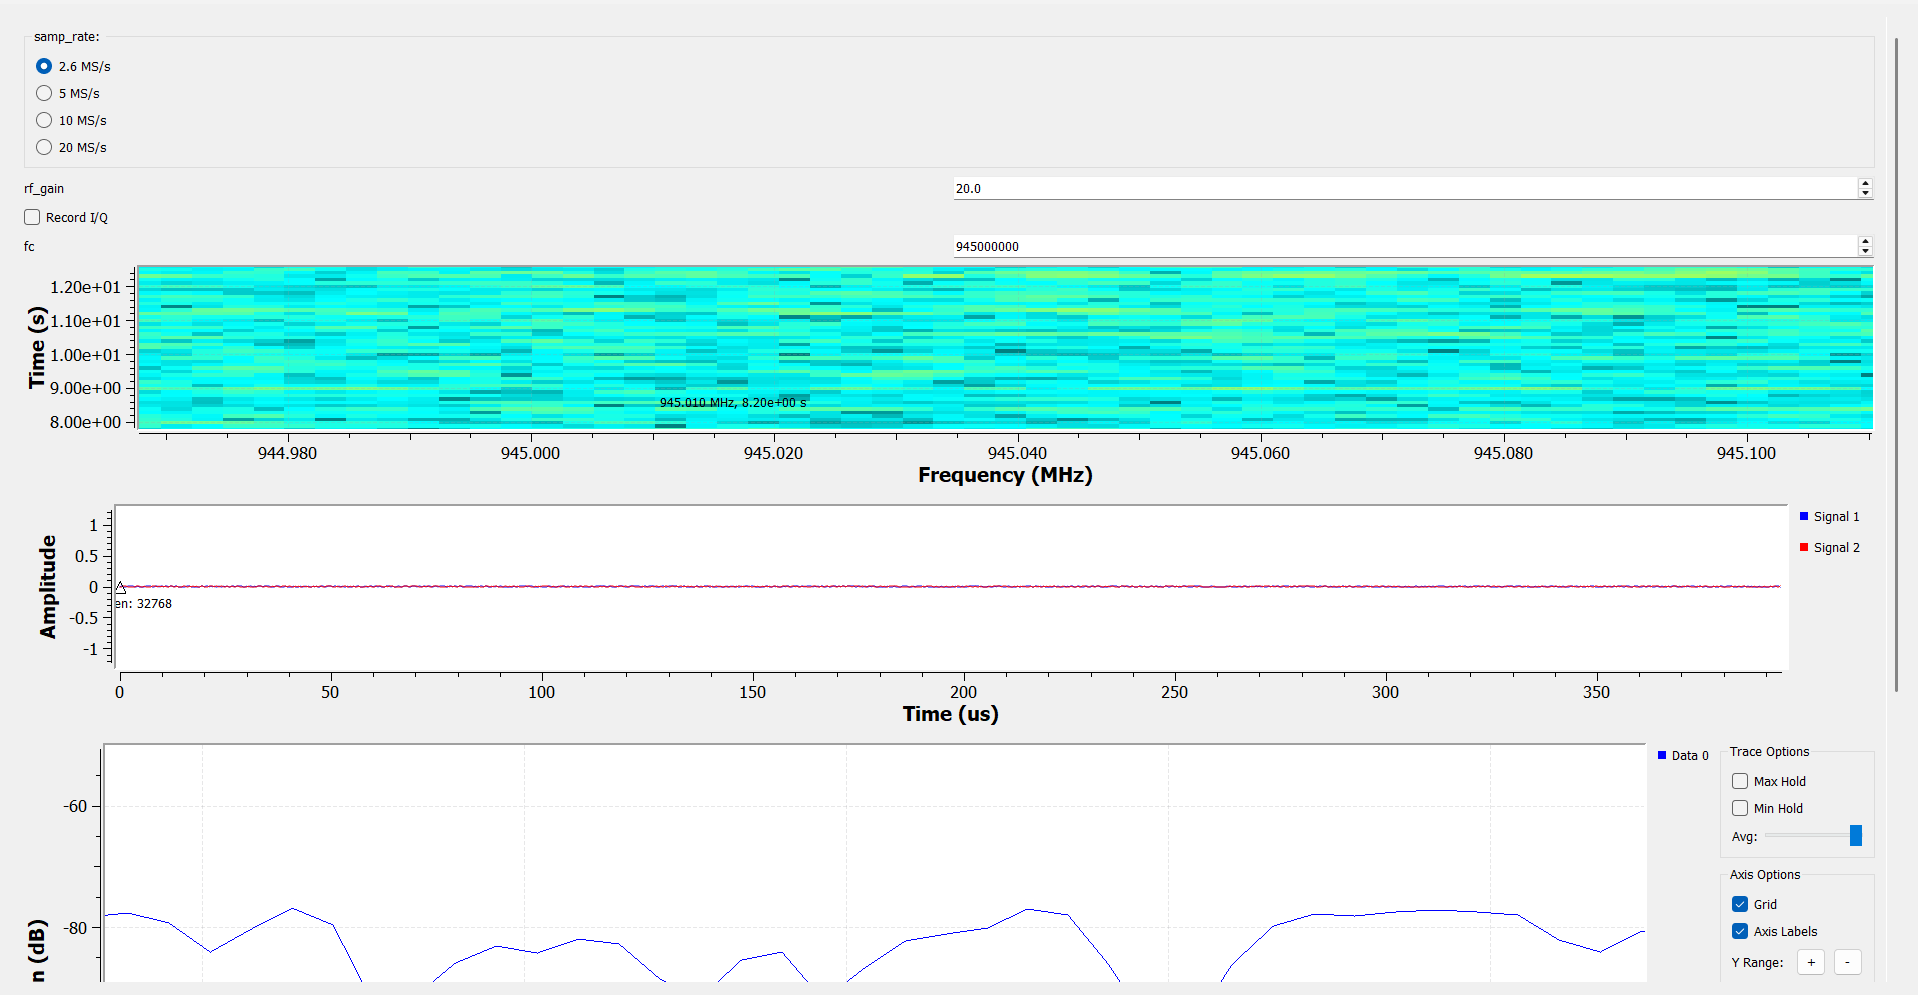
\includegraphics[width=0.96\linewidth,height=0.29\textheight,keepaspectratio]{../assets/images/lab01/P1_GSMcarriers.png}\caption{\rtl{نمای اولیهٔ باریک؛ برای اندازه‌گیری یک سیگنال چندمگاهرتزی کافی نیست.}}\label{fig:3}\end{figure}
\rp{تصویر ثبت‌شده در شکل \ref{fig:4} آمده است.}
\begin{figure}[H]\centering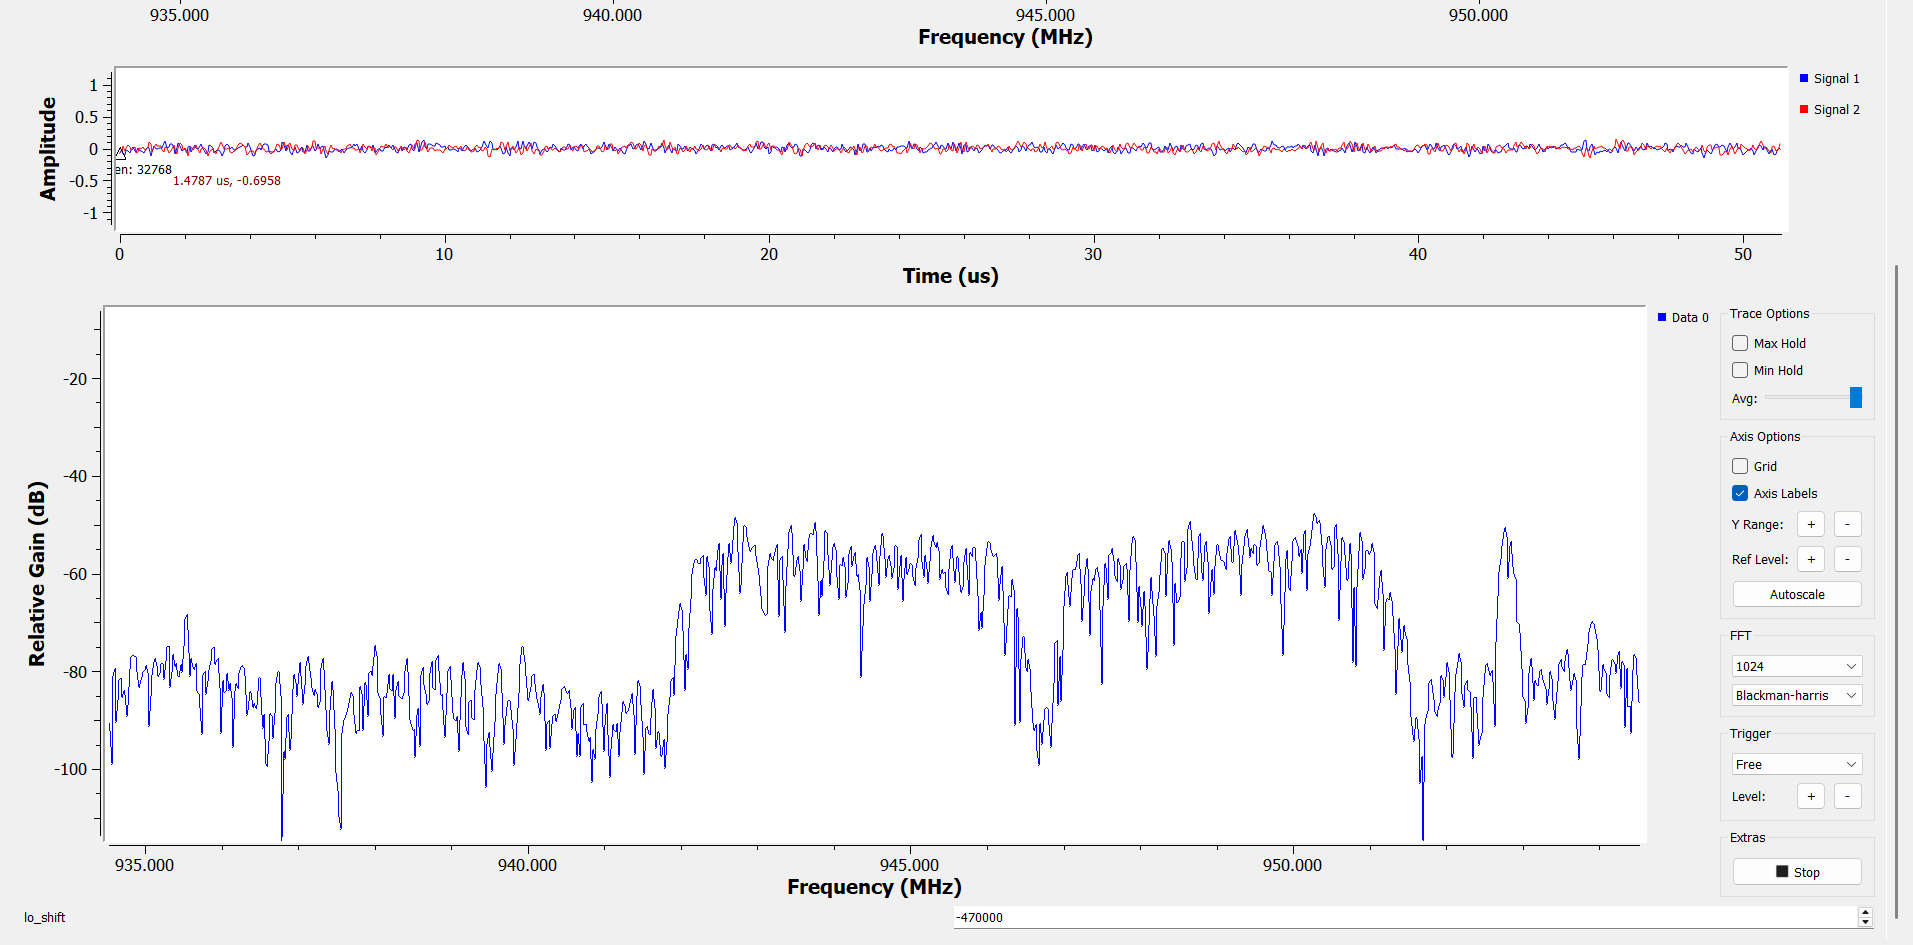
\includegraphics[width=0.96\linewidth,height=0.29\textheight,keepaspectratio]{../assets/images/lab01/P1_GSMcarriers_20MS_2.png}\caption{\rtl{نمای پهن و دو بلوک طیفی؛ مقدار \lr{lo\_shift} در پایین این تصویر \lr{−}۴۷۰۰۰۰۰ هرتز است و در تفسیر مرکز باید لحاظ شود.}}\label{fig:4}\end{figure}
\rp{تصویر ثبت‌شده در شکل \ref{fig:5} آمده است.}
\begin{figure}[H]\centering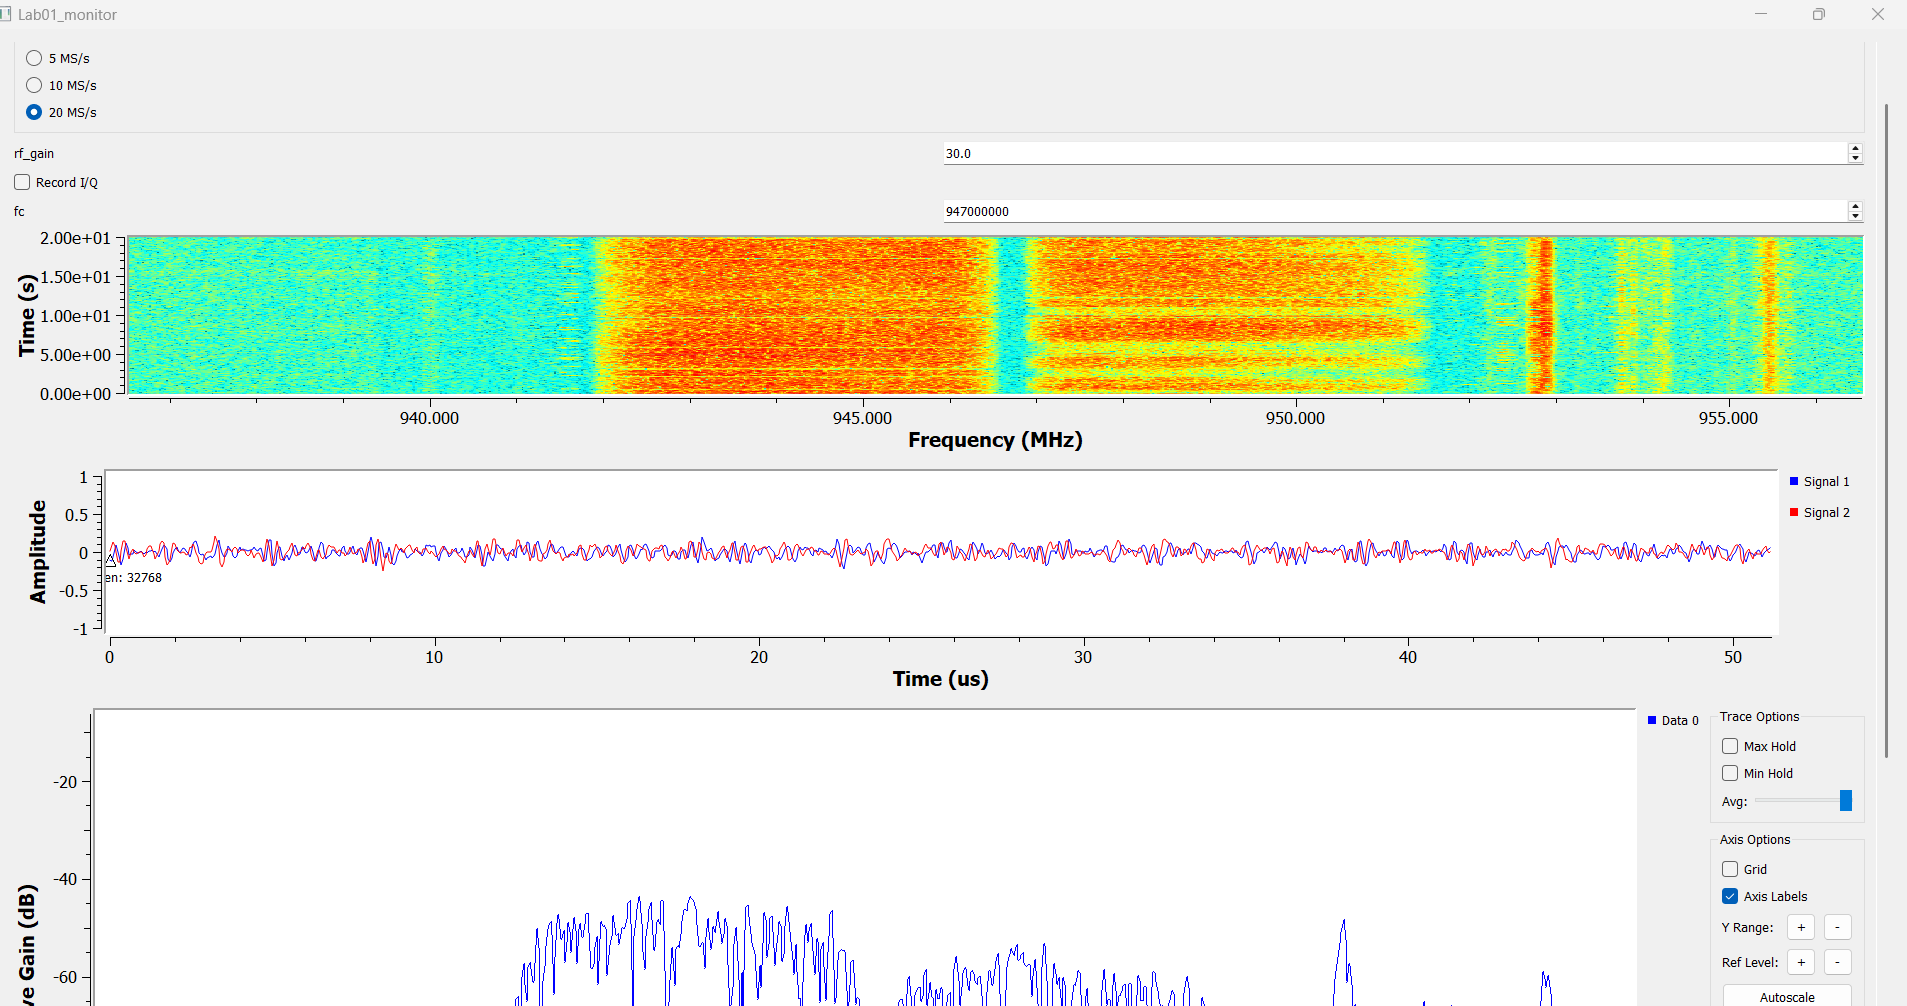
\includegraphics[width=0.96\linewidth,height=0.29\textheight,keepaspectratio]{../assets/images/lab01/P1_GSMcarriers_947.png}\caption{\rtl{ثبت دیگر پس از تغییر تنظیم مرکز؛ شکل کلی بلوک‌های پهن باقی می‌ماند.}}\label{fig:5}\end{figure}
\rp{در \lr{P3\_radio\_2} محور فرکانس حدود ۹۳۳ تا ۹۵۳ \lr{MHz} است. خوانش چشمی لبه‌ها، بلوک اول را تقریباً ۹۴۲ تا ۹۴۶٫۵ و بلوک دوم را تقریباً ۹۴۷ تا ۹۵۱٫۵ \lr{MHz} نشان می‌دهد: مراکز هندسی حدود ۹۴۴٫۲۵ و ۹۴۹٫۲۵ \lr{MHz} و عرض ظاهری هرکدام حدود ۴٫۵ \lr{MHz.} عدم قطعیت خوانش تصویر دست‌کم حدود ۰٫۲ \lr{MHz} است؛ این عرض، \lr{B6} یا \lr{B20} یا \lr{OBW99} اندازه‌گیری‌شده نیست. نزدیکی به عرض فعال \lr{LTE} پنج‌مگاهرتزی و لبه‌های تیز، فرضیهٔ \lr{LTE} را تقویت می‌کند، ولی \lr{UMTS} یا ترکیب سیگنال‌ها با این مدرک به‌طور قطعی رد نمی‌شود [۳،۴].}

\rp{تصویر ثبت‌شده در شکل \ref{fig:6} آمده است.}
\begin{figure}[H]\centering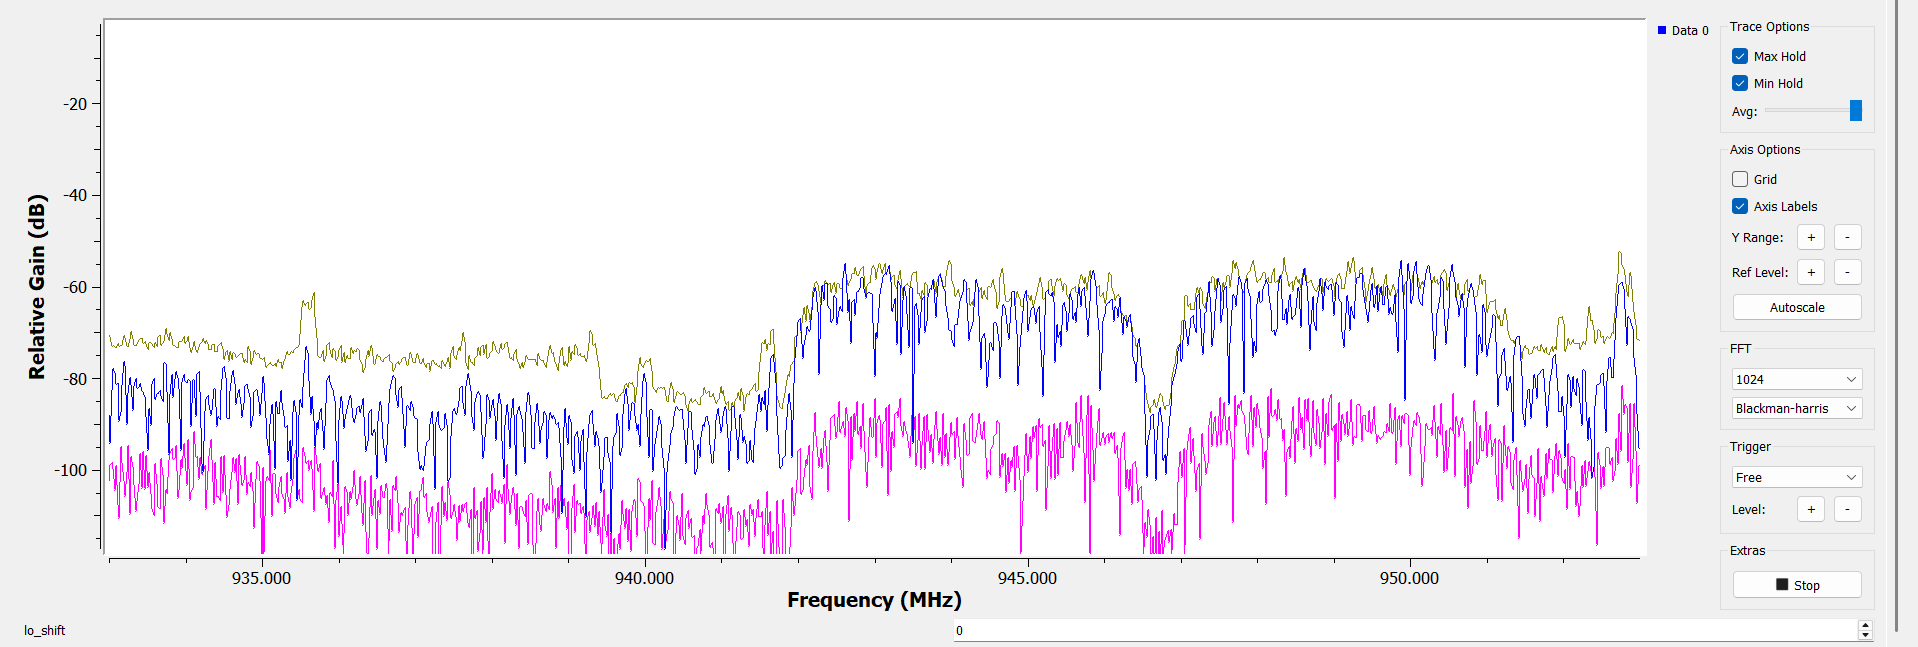
\includegraphics[width=0.96\linewidth,height=0.29\textheight,keepaspectratio]{../assets/images/lab01/P3_radio_2.png}\caption{\rtl{با وجود نام \lr{radio}، این تصویر باند سلولی ۹۰۰ مگاهرتز را نشان می‌دهد، نه پخش \lr{FM} در ۸۸ تا ۱۰۸ مگاهرتز.}}\label{fig:6}\end{figure}
\Needspace{6\baselineskip}
\section{\rtl{۳. آزمون حلقه، علامت فرکانس و جابه‌جایی LO}}
\rp{در فایل \lr{GRC} موجود، فرکانس \lr{TX} برابر \lr{int(fc)}، فرکانس \lr{RX} و محور هر دو برابر \lr{f\_tune=int(fc+lo\_shift)} و فرکانس تن برابر \lr{f\_tx} است. با \lr{fc=434 MHz} و \lr{f\_tx=+250 kHz}، انتظار تن در \lr{434.25 MHz} است. تصاویر تن قوی نزدیک این مقدار و با تغییر علامت، تن نزدیک \lr{433.75 MHz} را نشان می‌دهند.}

\rp{تصویر ثبت‌شده در شکل \ref{fig:7} آمده است.}
\begin{figure}[H]\centering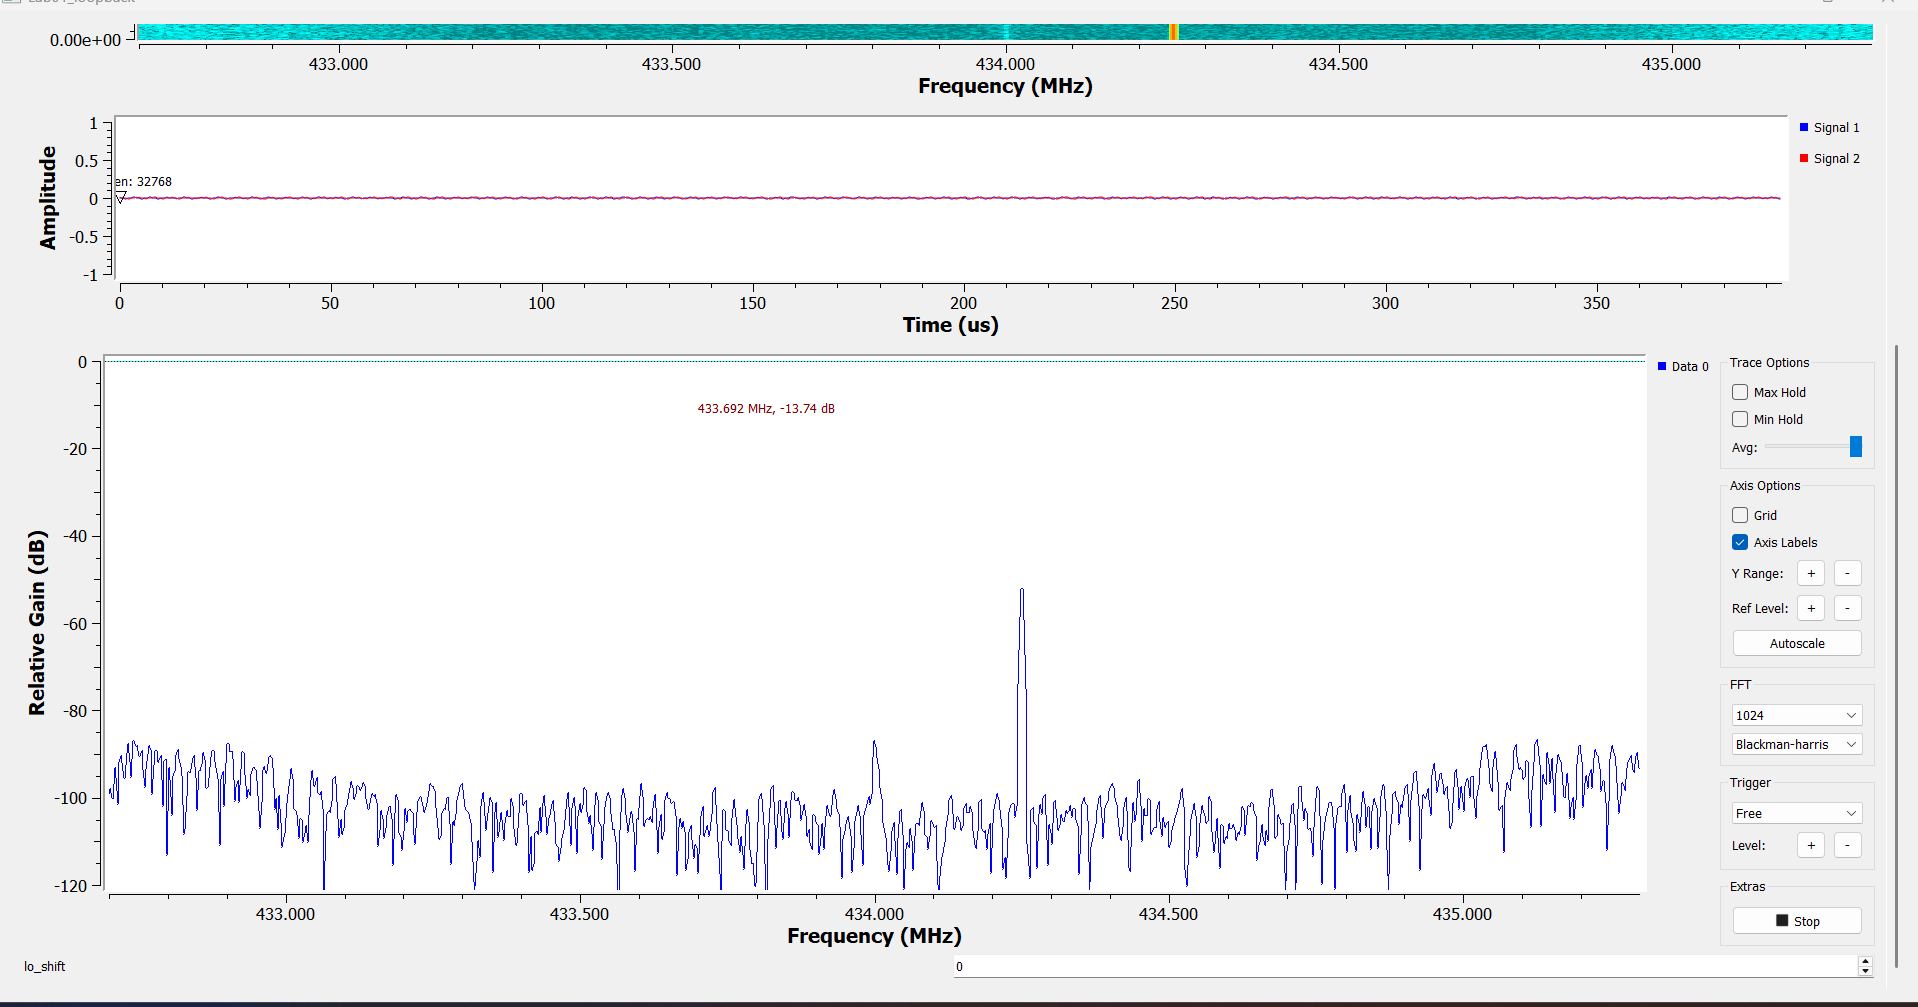
\includegraphics[width=0.96\linewidth,height=0.29\textheight,keepaspectratio]{../assets/images/lab01/P2_fc434_2.png}\caption{\rtl{تن مثبت نزدیک ۴۳۴٫۲۵ \lr{MHz} با \lr{lo\_shift=0}؛ متن قرمز نشانگر ماوس است و الزاماً روی قله قرار ندارد.}}\label{fig:7}\end{figure}
\rp{تصویر ثبت‌شده در شکل \ref{fig:8} آمده است.}
\begin{figure}[H]\centering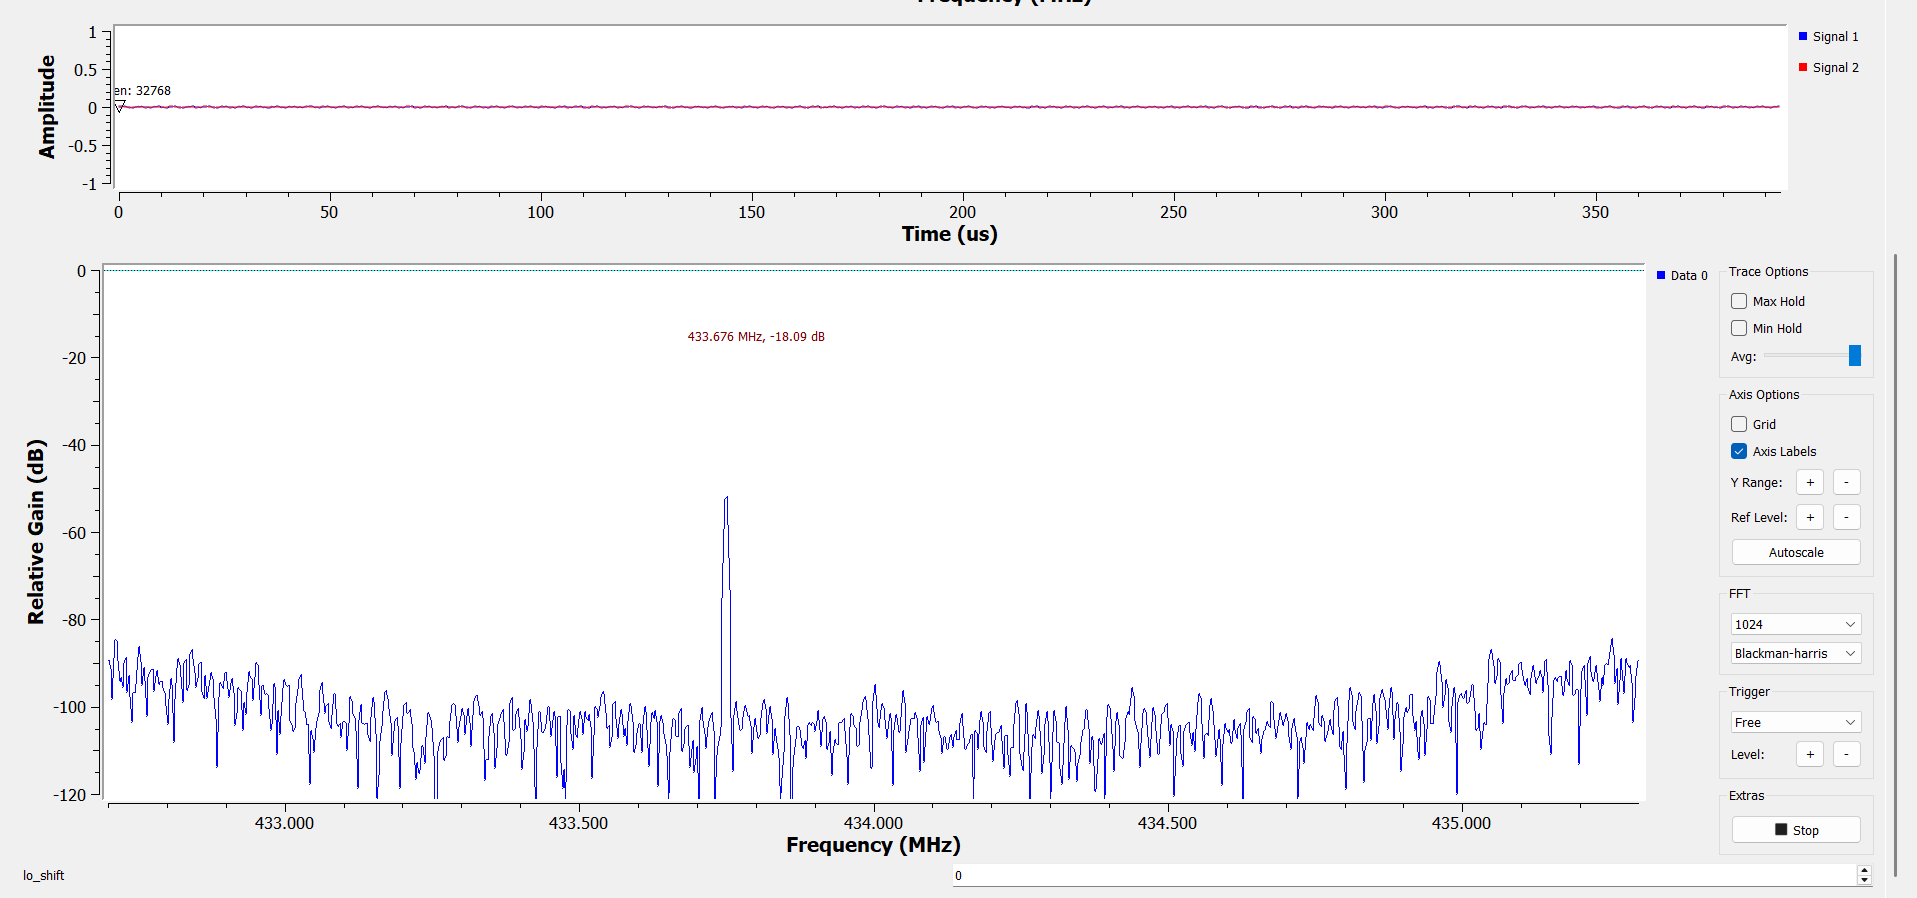
\includegraphics[width=0.96\linewidth,height=0.29\textheight,keepaspectratio]{../assets/images/lab01/P2_fc434_txInverted_3.png}\caption{\rtl{با فرکانس مختلط منفی، تن در سمت چپ مرکز و نزدیک ۴۳۳٫۷۵ \lr{MHz} قرار می‌گیرد.}}\label{fig:8}\end{figure}
\rp{جدول \ref{tab:lo} اطلاعات این بخش را ثبت می‌کند.}
\begin{table}[H]\centering\small\renewcommand{\arraystretch}{1.25}
\begin{tabular}{|p{0.21\linewidth}|p{0.21\linewidth}|p{0.21\linewidth}|p{0.21\linewidth}|}\hline
\rtl{\textbf{تصویر \lr{RX} از تن (\lr{MHz)}}} & \rtl{\textbf{\lr{DC} گیرنده (\lr{MHz)}}} & \rtl{\textbf{تن واقعی (\lr{MHz)}}} & \rtl{\textbf{\lr{lo\_shift (kHz)}}} \\ \hline
\rtl{\lr{433.550}} & \rtl{\lr{433.900}} & \rtl{\lr{434.250}} & \rtl{\lr{−100}} \\ \hline
\rtl{\lr{433.750}} & \rtl{\lr{434.000}} & \rtl{\lr{434.250}} & \rtl{\lr{0}} \\ \hline
\rtl{\lr{433.950}} & \rtl{\lr{434.100}} & \rtl{\lr{434.250}} & \rtl{+\lr{100}} \\ \hline
\rtl{\lr{434.150}} & \rtl{\lr{434.200}} & \rtl{\lr{434.250}} & \rtl{+\lr{200}} \\ \hline
\end{tabular}\caption{\rtl{انتظار تئوری آزمون \lr{LO} برای تن مثبت؛ این جدول اندازه‌گیری قله‌ها نیست}}\label{tab:lo}\end{table}
\rp{در تصاویر \lr{lo\_shift=+100}، +\lr{200} و \lr{−100}، قلهٔ اصلی نزدیک ۴۳۴٫۲۵ تا ۴۳۴٫۳۰ \lr{MHz} باقی می‌ماند؛ پس مشاهدهٔ کیفی با ثابت‌ماندن \lr{RF} تن سازگار است. چند قلهٔ جانبی هم دیده می‌شود، اما همهٔ آن‌ها با الگوی سادهٔ \lr{DC} یا تصویر آینه‌ای \lr{RX} در جدول بالا منطبق نیستند. به‌خصوص جابه‌جایی بعضی قله‌های جانبی بزرگ‌تر از انتظار است. آن‌ها را بدون بازخوانی هم‌زمان \lr{RX LO}، \lr{TX LO} و نرخ، «حامل واقعی» یا «نشتی مشخص» نام‌گذاری قطعی نمی‌کنیم.}

\rp{تصویر ثبت‌شده در شکل \ref{fig:9} آمده است.}
\begin{figure}[H]\centering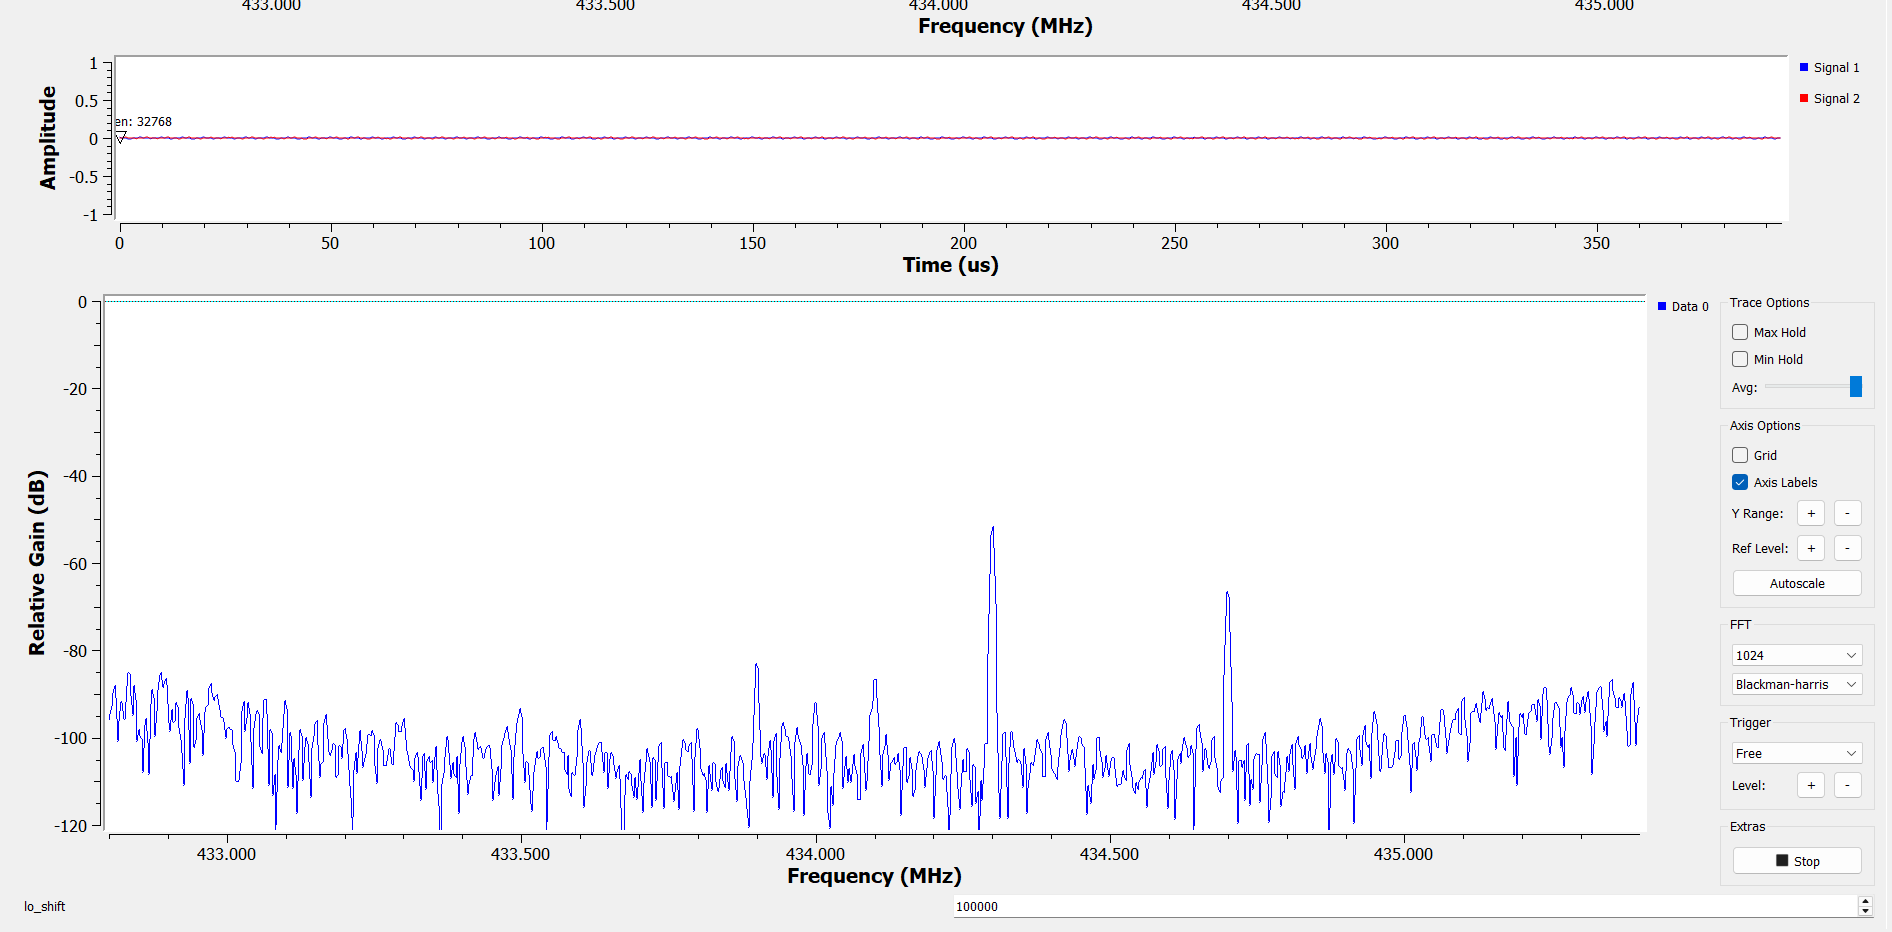
\includegraphics[width=0.96\linewidth,height=0.29\textheight,keepaspectratio]{../assets/images/lab01/P2_flo_100_2.png}\caption{\rtl{آزمون جابه‌جایی +۱۰۰ \lr{kHz}؛ قله‌های جانبی نیازمند تطبیق با دادهٔ خام و تنظیمات واقعی‌اند.}}\label{fig:9}\end{figure}
\rp{تصویر ثبت‌شده در شکل \ref{fig:10} آمده است.}
\begin{figure}[H]\centering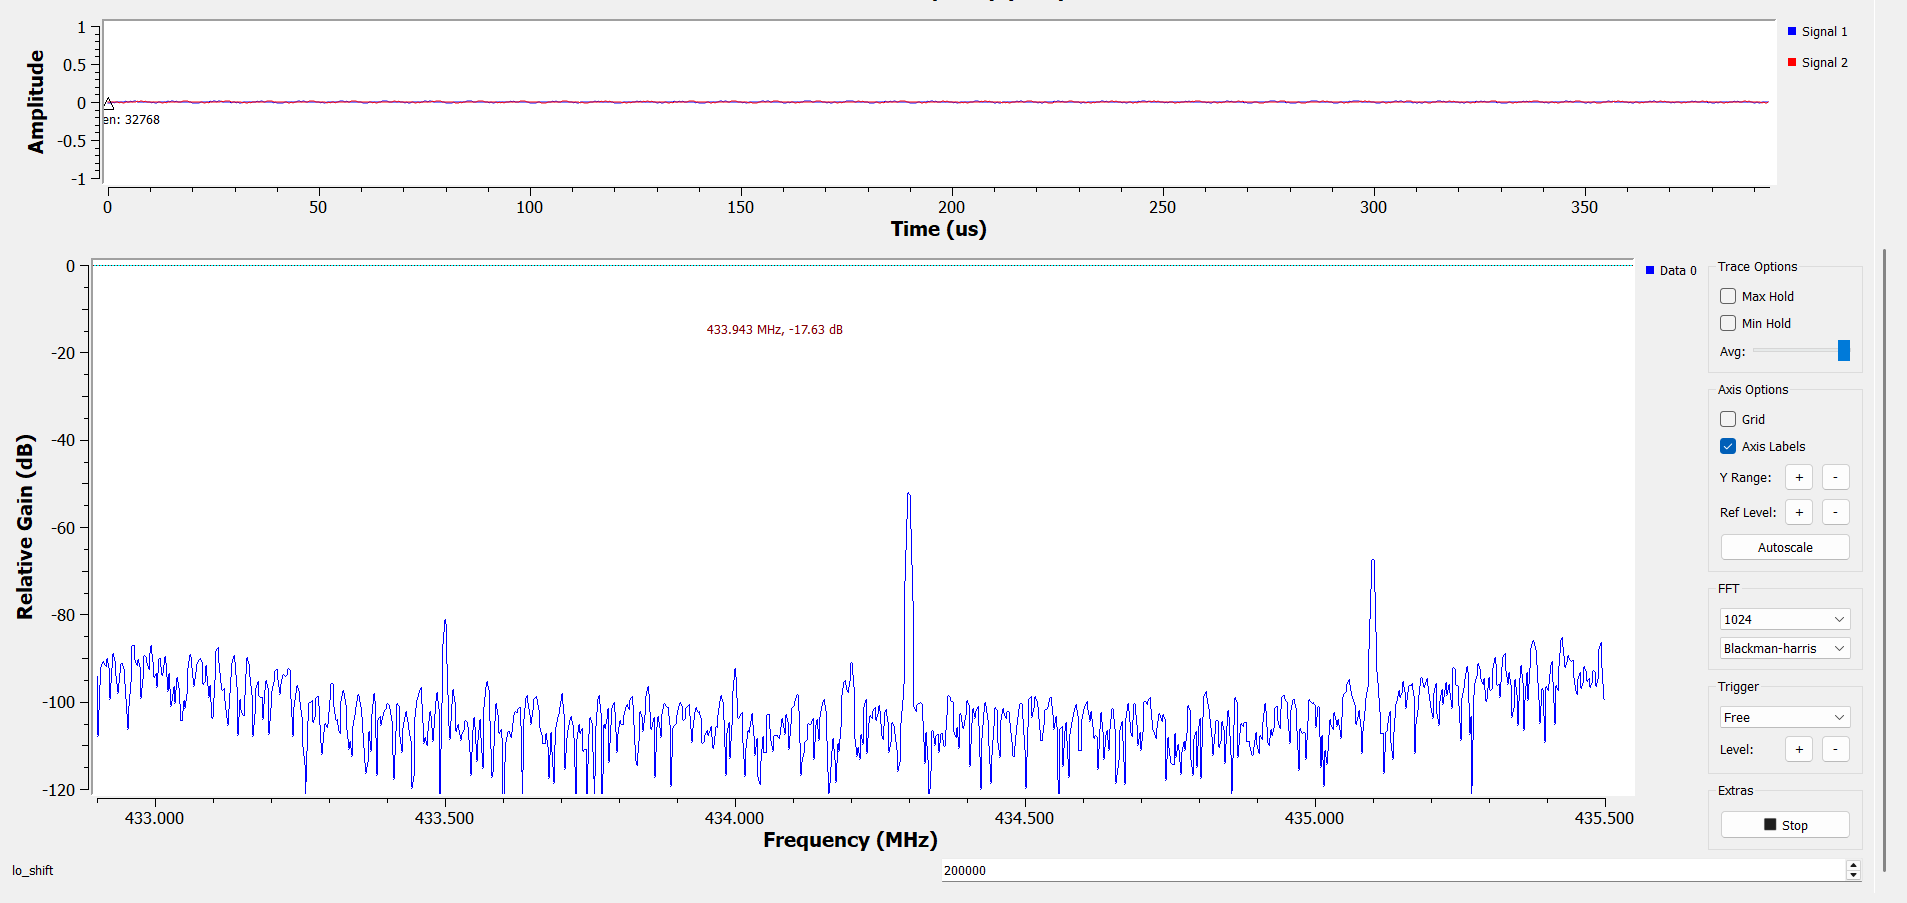
\includegraphics[width=0.96\linewidth,height=0.29\textheight,keepaspectratio]{../assets/images/lab01/P2_f_lo_200.png}\caption{\rtl{آزمون +۲۰۰ \lr{kHz}؛ عدد قرمز \lr{433.943 MHz} محل ماوس است، نه برآورد قلهٔ تن.}}\label{fig:10}\end{figure}
\rp{تصویر ثبت‌شده در شکل \ref{fig:11} آمده است.}
\begin{figure}[H]\centering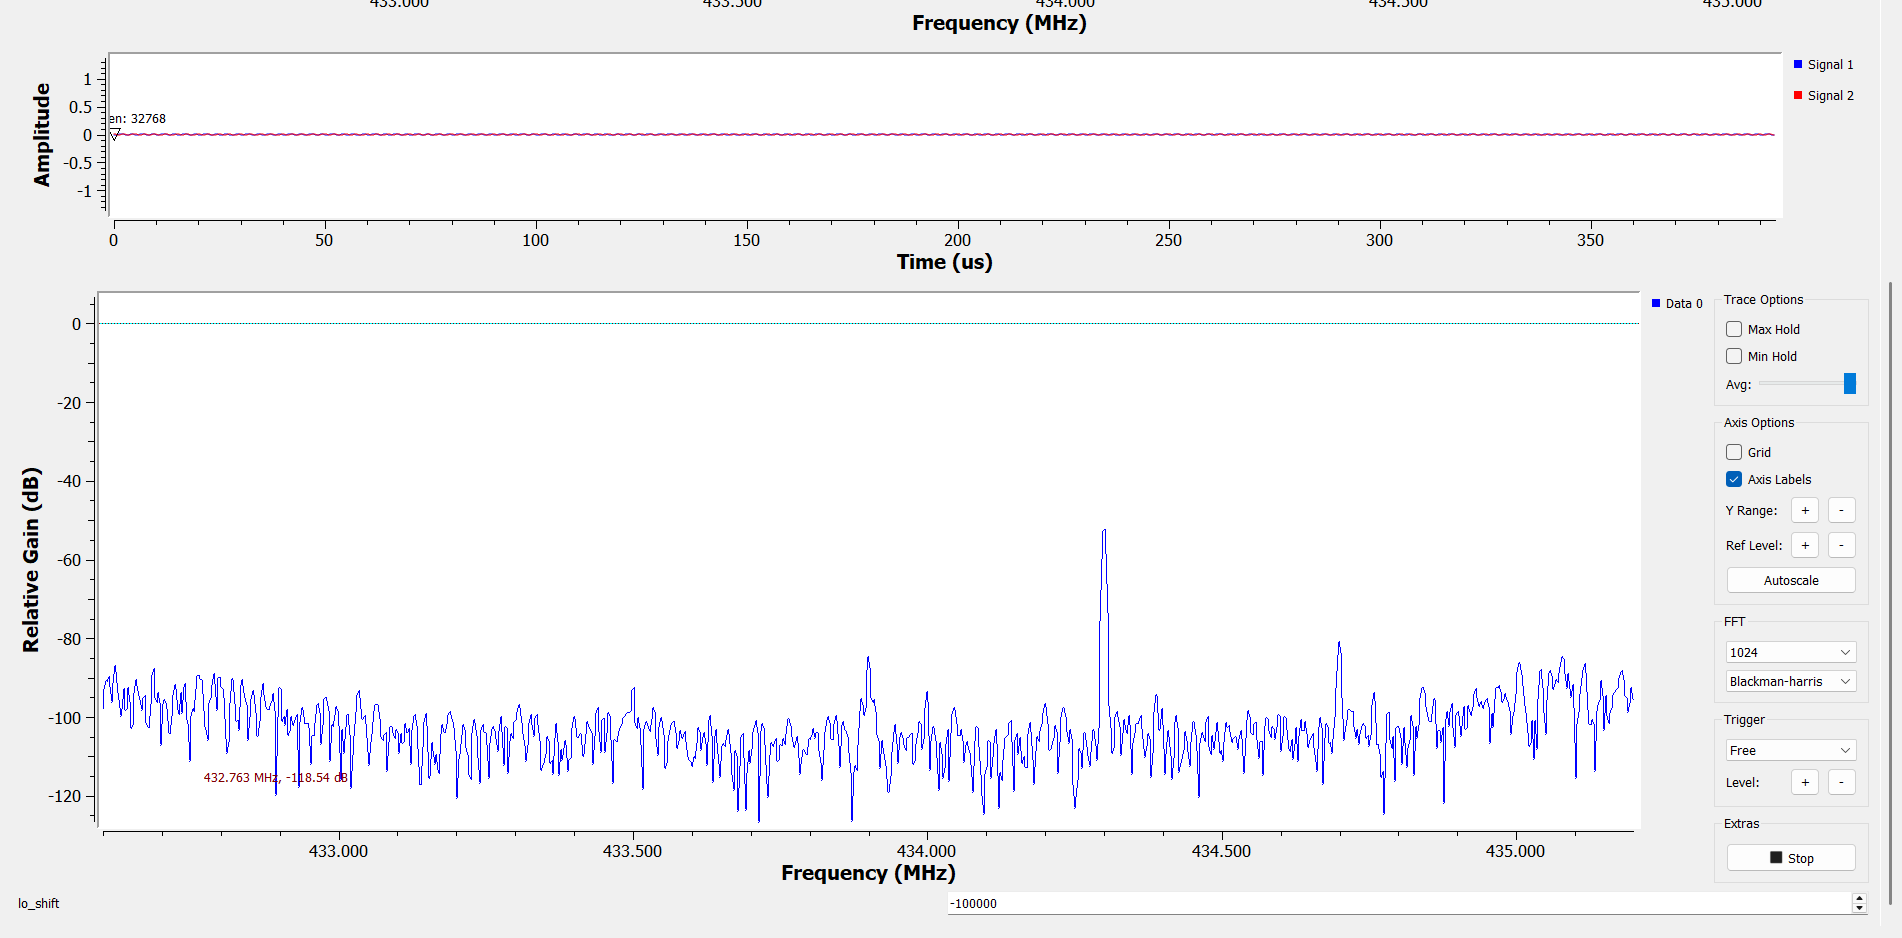
\includegraphics[width=0.96\linewidth,height=0.29\textheight,keepaspectratio]{../assets/images/lab01/P2_f_lo_-100_2.png}\caption{\rtl{آزمون \lr{−}۱۰۰ \lr{kHz}؛ اصلی و قله‌های ضعیف باید به صورت یک دنبالهٔ آزمون تحلیل شوند.}}\label{fig:11}\end{figure}
\rp{در \lr{P2\_DCoff} محور به حوالی ۹۴۵ \lr{MHz} تغییر کرده است؛ با این تصویر نمی‌توان افزایش قله را به خاموش‌شدن تصحیح \lr{DC} در ۴۳۴ \lr{MHz} نسبت داد. برای مقایسهٔ معتبر، باید دو ثبت با \lr{fc}، \lr{fs}، بهره، تضعیف و اتصال یکسان و فقط تغییر گزینه‌های \lr{DC} فراهم شود.}

\rp{تصویر ثبت‌شده در شکل \ref{fig:12} آمده است.}
\begin{figure}[H]\centering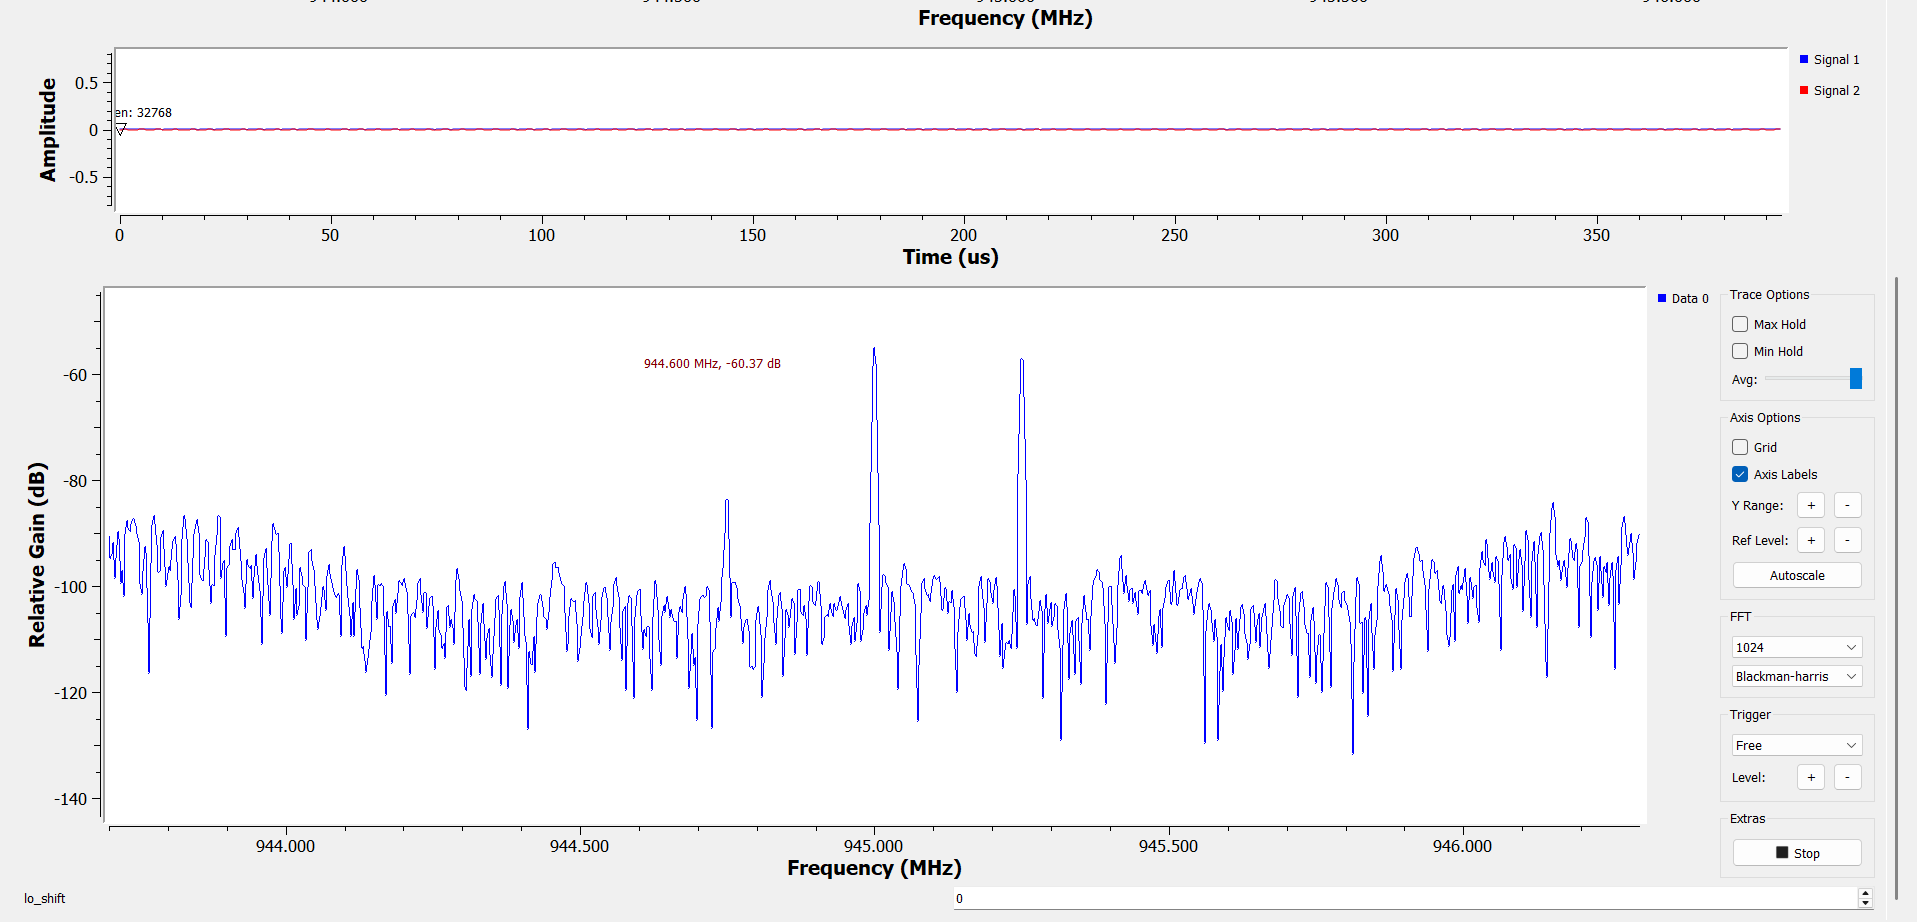
\includegraphics[width=0.96\linewidth,height=0.29\textheight,keepaspectratio]{../assets/images/lab01/P2_DCoff.png}\caption{\rtl{آزمون نام‌گذاری‌شدهٔ \lr{DCoff} با محور ۹۴۵ \lr{MHz}؛ ناسازگاری تنظیمات باید در نسخهٔ نهایی روشن شود.}}\label{fig:12}\end{figure}
\Needspace{6\baselineskip}
\section{\rtl{۴. پویش، ریموت و فراسوی تلفن}}
\rp{طبق دستور کار، در ۲۰ \lr{MS/s} فقط بخش مرکزی ۱۶ \lr{MHz} معتبر فرض می‌شود. برای فروسو مراکز ۹۴۳ و ۹۵۹ و برای فراسو ۸۹۸ و ۹۱۴ \lr{MHz} لازم‌اند. تصاویر موجود پوشش همهٔ گام‌ها را اثبات نمی‌کنند. در نمای فراسو حدود ۹۰۴ تا ۹۲۴ \lr{MHz}، تنها بخش داخل باند ۸۹۰ تا ۹۱۵ برای این تمرین فراسوی \lr{GSM900} است؛ قله‌های بالاتر از ۹۱۵ \lr{MHz} را به این سرویس نسبت نمی‌دهیم.}

\rp{در باند ریموت، تصویر خاموش عمدتاً کف طیف را نشان می‌دهد و تصویر روشن یک قلهٔ گذرا نزدیک ۴۳۳٫۹ \lr{MHz} ثبت می‌کند. فاصلهٔ زیاد \lr{Max Hold} از منحنی لحظه‌ای نشانهٔ رویدادی است که در قاب فعلی حضور ندارد. شکل، با ریموت \lr{OOK/FSK} سازگار است؛ تمایز این دو مدولاسیون و شمارش بسته‌ها از این تصاویر ممکن نیست. قله‌ها و دامن پهن در ثبت ۲۰ \lr{MS/s} می‌توانند اثر غیرخطی یا تداخل هم باشند و پهنای واقعی ریموت محسوب نمی‌شوند.}

\rp{تصویر ثبت‌شده در شکل \ref{fig:13} آمده است.}
\begin{figure}[H]\centering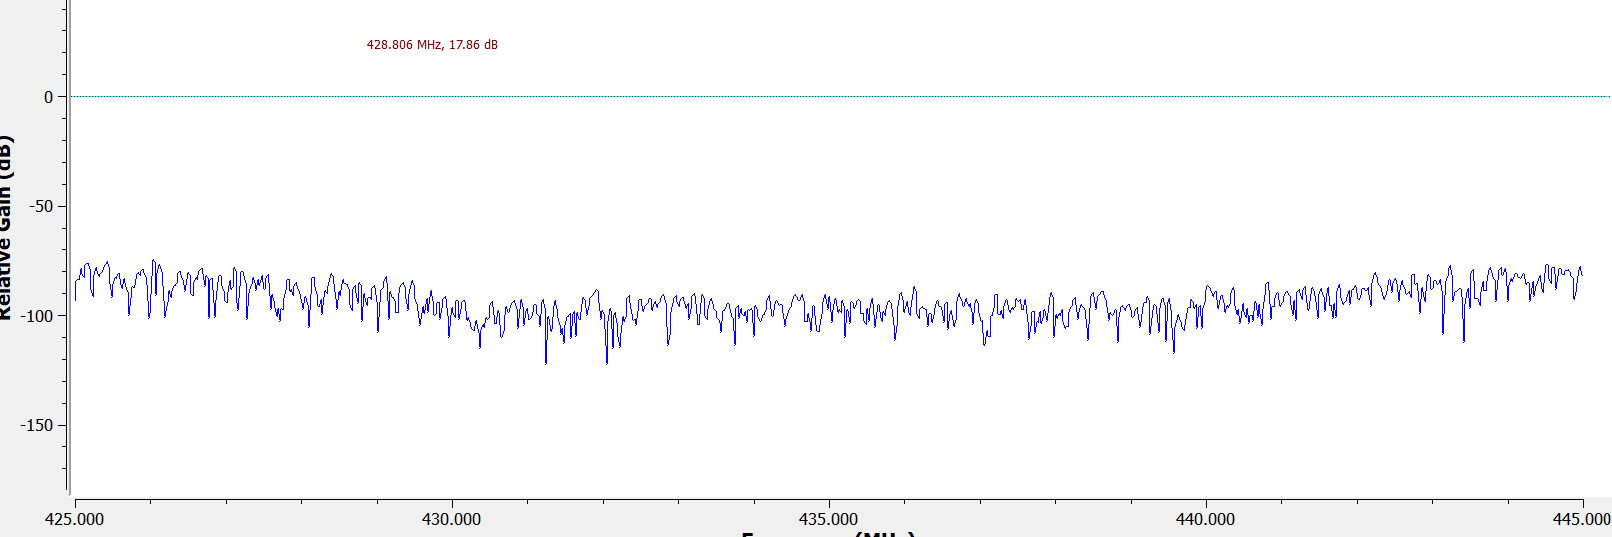
\includegraphics[width=0.96\linewidth,height=0.29\textheight,keepaspectratio]{../assets/images/lab01/P3_remote_off.png}\caption{\rtl{حالت بدون فشردن ریموت؛ مرجع مقایسهٔ طیف.}}\label{fig:13}\end{figure}
\rp{تصویر ثبت‌شده در شکل \ref{fig:14} آمده است.}
\begin{figure}[H]\centering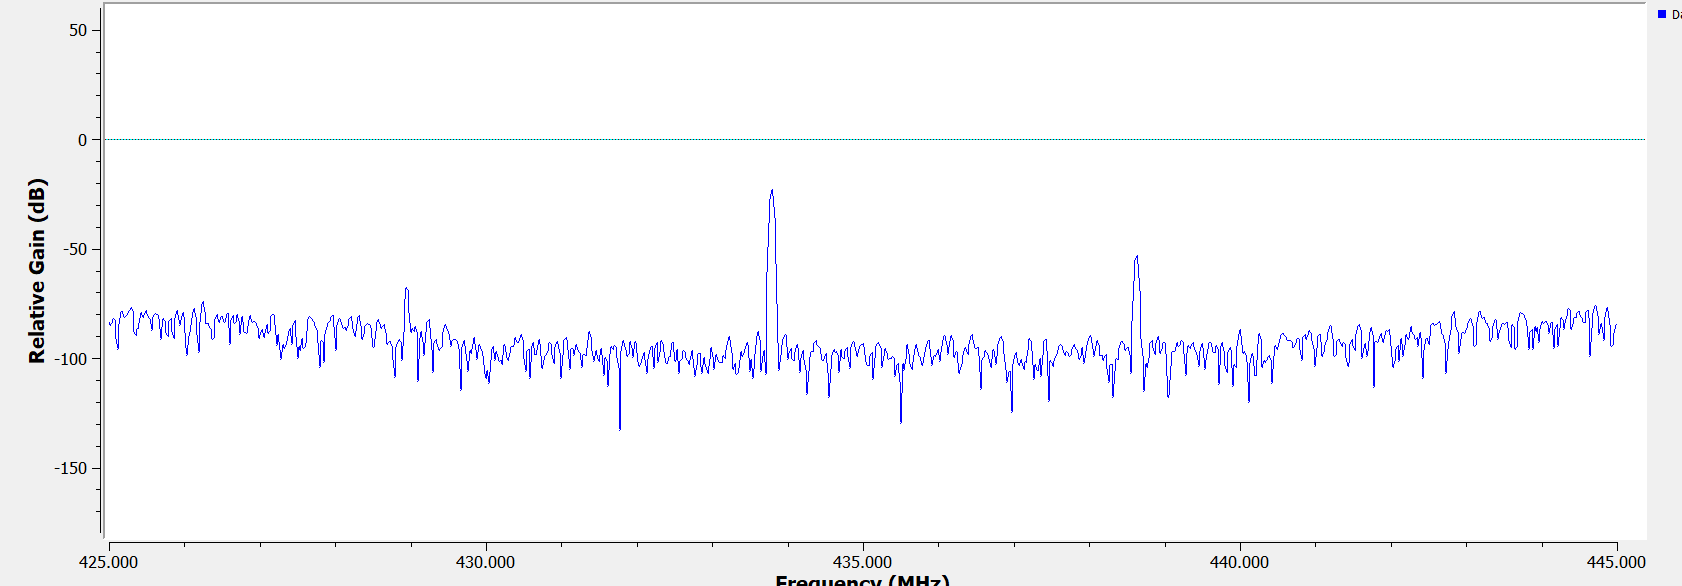
\includegraphics[width=0.96\linewidth,height=0.29\textheight,keepaspectratio]{../assets/images/lab01/P3_remote_on.png}\caption{\rtl{ثبت سیگنال هنگام فعال‌شدن ریموت؛ مقایسه باید با بهره و تنظیم یکسان تکمیل شود.}}\label{fig:14}\end{figure}
\rp{تصویر ثبت‌شده در شکل \ref{fig:15} آمده است.}
\begin{figure}[H]\centering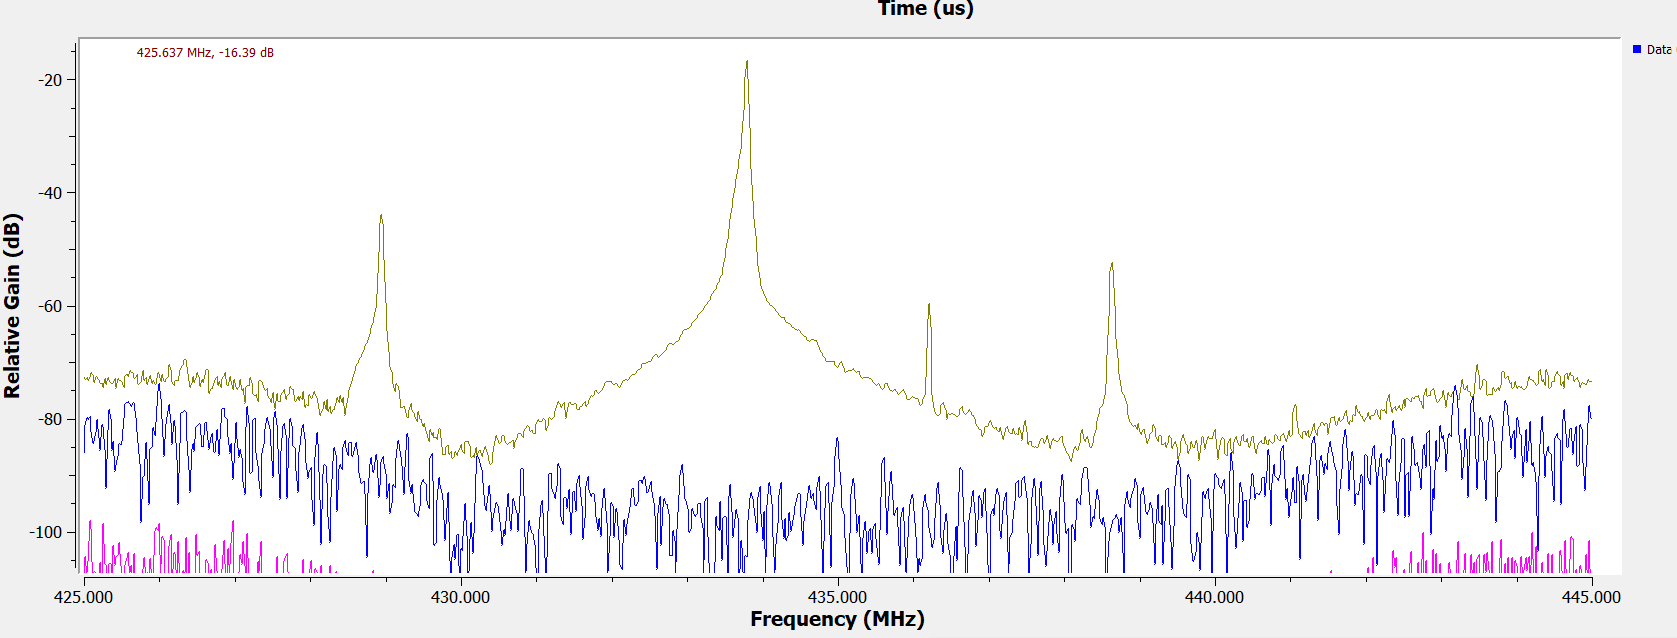
\includegraphics[width=0.96\linewidth,height=0.29\textheight,keepaspectratio]{../assets/images/lab01/P3_remote3.png}\caption{\rtl{\lr{Max Hold} اثر گذرا را نگه داشته است؛ دامن پهن و قله‌های دور نیاز به آزمون کاهش بهره دارند.}}\label{fig:15}\end{figure}
\rp{پس از تماس، \lr{Max Hold} در حوالی ۹۰۷ تا ۹۰۹ و نزدیک ۹۱۱٫۶ \lr{MHz} افزایش‌هایی را ثبت کرده که در نمای بدون تماس به این قوت دیده نمی‌شوند. آبشار نیز رگه‌های زمانی محدود نشان می‌دهد. این شواهد با ارسال برستی تلفن سازگارند؛ اتصال فقط نسل دو و وابستگی دقیق هر قله به تلفن گروه در مدارک تأیید نشده است.}

\rp{تصویر ثبت‌شده در شکل \ref{fig:16} آمده است.}
\begin{figure}[H]\centering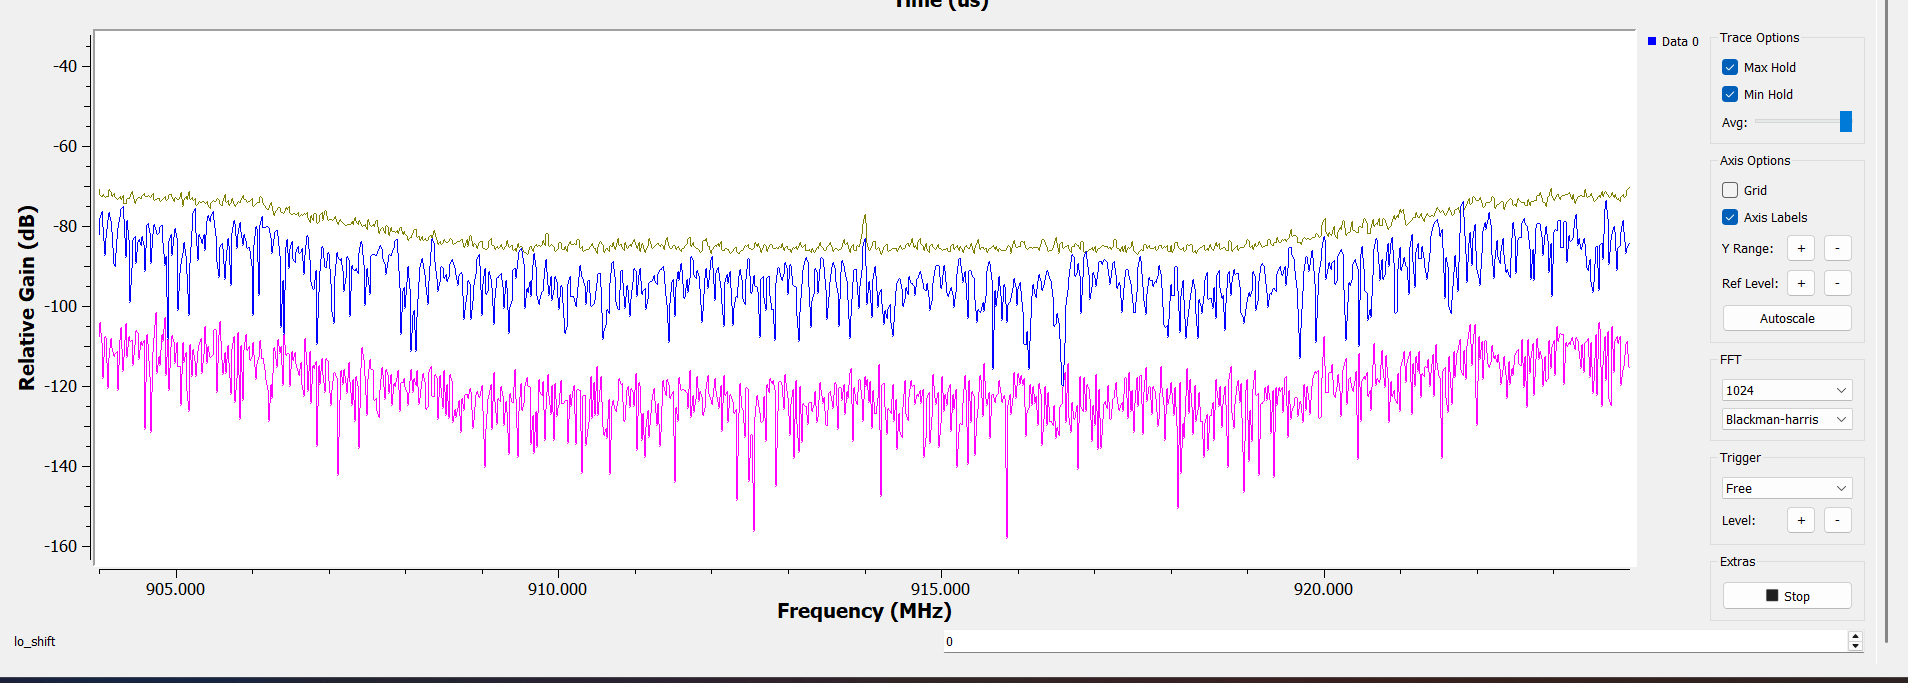
\includegraphics[width=0.96\linewidth,height=0.29\textheight,keepaspectratio]{../assets/images/lab01/P3_GSMuplink_noCall.png}\caption{\rtl{پیش از تماس: منحنی لحظه‌ای و حافظهٔ نگه‌داشتن قله‌ها.}}\label{fig:16}\end{figure}
\rp{تصویر ثبت‌شده در شکل \ref{fig:17} آمده است.}
\begin{figure}[H]\centering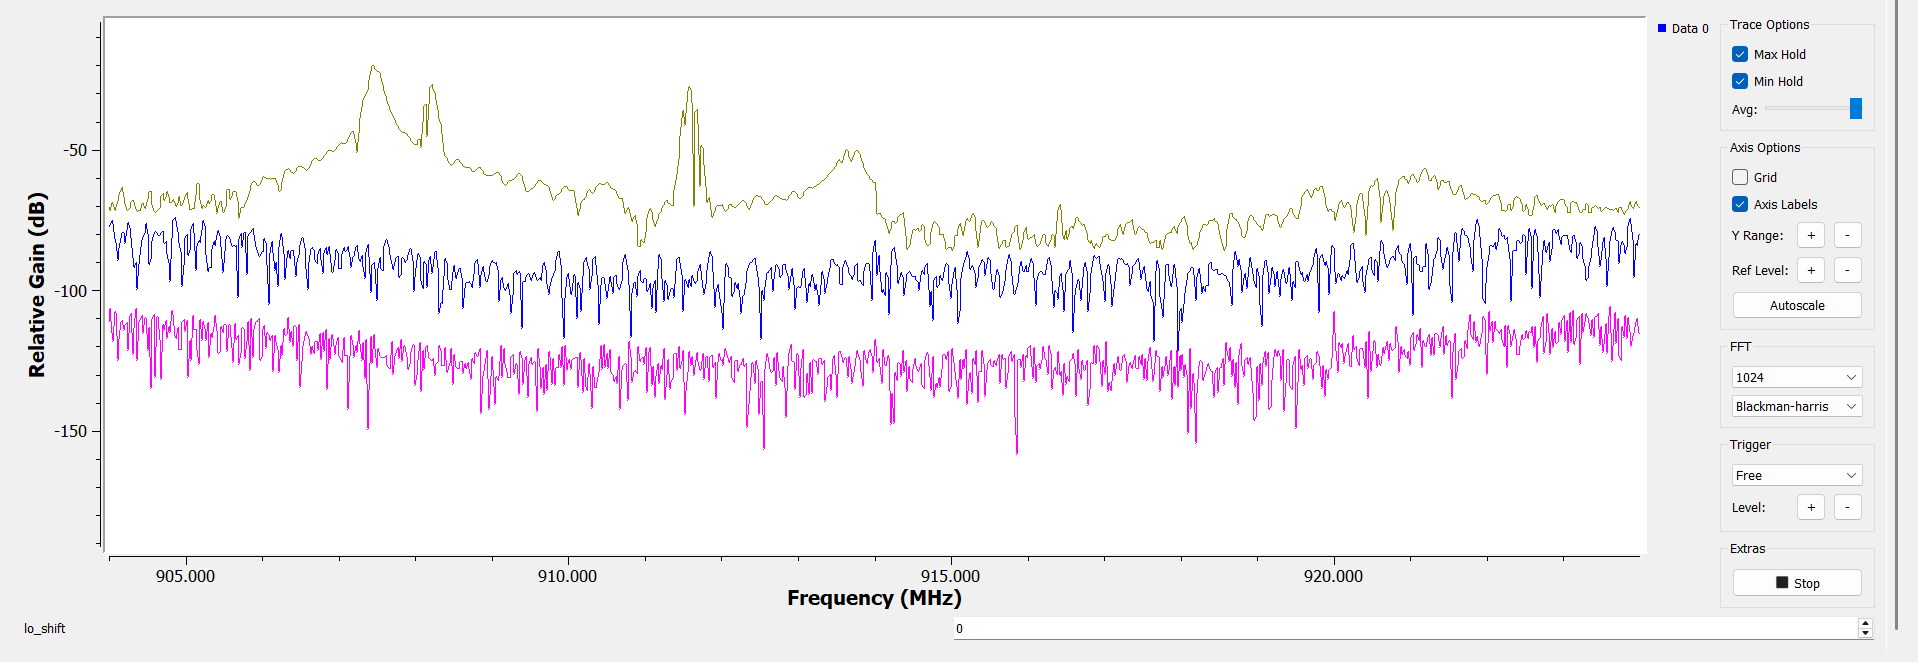
\includegraphics[width=0.96\linewidth,height=0.29\textheight,keepaspectratio]{../assets/images/lab01/P3_GSMuplink_afterCall.png}\caption{\rtl{پس از تماس: افزایش فعالیت گذرا در بخشی از باند فراسو.}}\label{fig:17}\end{figure}
\rp{تصویر ثبت‌شده در شکل \ref{fig:18} آمده است.}
\begin{figure}[H]\centering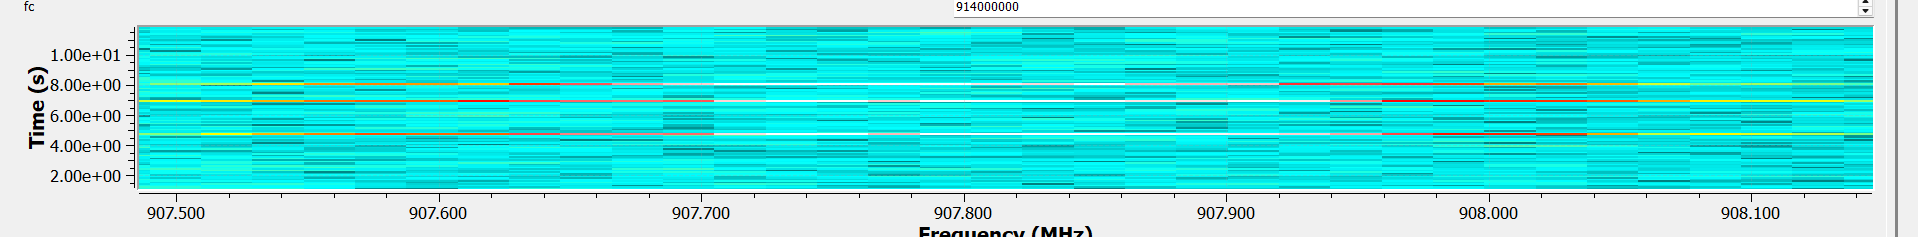
\includegraphics[width=0.96\linewidth,height=0.29\textheight,keepaspectratio]{../assets/images/lab01/P3_GSMuplink_waterfallBursts.png}\caption{\rtl{ردهای گذرا در آبشار؛ محور زمان نمایشگر زنده برای اندازه‌گیری مدت برست کافی نیست.}}\label{fig:18}\end{figure}
\Needspace{6\baselineskip}
\section{\rtl{۵. فهرست سیگنال‌ها و پیش‌بینی در برابر مشاهده}}
\rp{جدول \ref{tab:inventory} اطلاعات این بخش را ثبت می‌کند.}
\begin{table}[H]\centering\small\renewcommand{\arraystretch}{1.25}
\begin{tabular}{|p{0.288\linewidth}|p{0.288\linewidth}|p{0.288\linewidth}|}\hline
\rtl{\textbf{پیش‌بینی / نتیجه}} & \rtl{\textbf{فرکانس و رفتار}} & \rtl{\textbf{نامزد / باند}} \\ \hline
\rtl{\lr{OOK/FSK} محتمل؛ پهنا از \lr{IQ} و فایل متناظر لازم است} & \rtl{حدود ۴۳۳٫۹۲ \lr{MHz}، گذرا} & \rtl{ریموت / ب} \\ \hline
\rtl{\lr{LTE} پنج‌مگاهرتزی محتمل؛ \lr{Bx} و \lr{OBW99} هنوز محاسبه نشده} & \rtl{مرکز حدود ۹۴۴٫۲۵ \lr{MHz}، عرض ظاهری ۴٫۵ \lr{MHz}، ماندگار} & \rtl{بلوک پهن ۱ / ج فروسو} \\ \hline
\rtl{\lr{LTE} پنج‌مگاهرتزی محتمل؛ فناوری نیازمند شاهد تکمیلی} & \rtl{مرکز حدود ۹۴۹٫۲۵ \lr{MHz}، عرض ظاهری ۴٫۵ \lr{MHz}، ماندگار} & \rtl{بلوک پهن ۲ / ج فروسو} \\ \hline
\rtl{ارسال سلولی محتمل؛ استقلال و پهنای کانال نیازمند \lr{IQ}} & \rtl{حدود ۹۰۸٫۲ \lr{MHz}، در \lr{Max Hold} پس از تماس} & \rtl{فعالیت فراسو ۱ / ج(۲)} \\ \hline
\rtl{\lr{GSM} محتمل؛ فعلاً حامل مستقل تأییدشده نیست} & \rtl{حدود ۹۱۱٫۶ \lr{MHz}، گذرا} & \rtl{فعالیت فراسو ۲ / ج(۲)} \\ \hline
\end{tabular}\caption{\rtl{پنج نامزد برای تحلیل؛ همهٔ مقادیر فرکانسی این جدول تقریب تصویری‌اند}}\label{tab:inventory}\end{table}
\rp{این پنج ردیف، پنج اندازه‌گیری کامل طبق جدول ۷ نیستند. سه محدودهٔ باند ب، ج فروسو و ج(۲) فراسو نماینده دارند و گذرا و پهن نیز دیده شده، اما برای احراز الزام درس، جدایی سیگنال‌ها، \lr{fL}، \lr{fU}، مقدار \lr{x}، سطح قله، \lr{fs} و نام فایل هر ردیف باید از دادهٔ خام تکمیل شود. سیگنال حلقه جای یکی از پنج سیگنال واقعی محیط را نمی‌گیرد.}

\rp{برای \lr{LTE} پنج‌مگاهرتزی، ۲۵ بلوک منبع با عرض هر بلوک ۱۸۰ \lr{kHz} پهنای پیکربندی فعال ۴٫۵ \lr{MHz} می‌دهد [۳]. توافق تقریبی عرض چشمی با این مقدار فقط قرینهٔ تشخیص است؛ مقایسهٔ خطای نسبی \lr{OBW99} با پهنای اسمی کانال بدون تعریف مشترک معتبر نیست. برای مقایسهٔ نهایی از |\lr{B\_measured−B\_reference}|/\lr{B\_reference} استفاده می‌کنیم و نوع پهنا را صریح یکسان می‌گیریم. برای ریموت، مدل و پهنای مرجع سازنده در دست نیست؛ برای \lr{GSM} نیز فاصلهٔ شبکهٔ کانال ۲۰۰ \lr{kHz} الزاماً \lr{B99} نیست.}

\rp{برای \lr{FM} مدرک باند صحیح موجود نیست؛ تعداد ایستگاه و پهنای آن گزارش نمی‌شود. پیش‌بینی \lr{GSM} باریک در برابر مشاهدهٔ بلوک‌های پهن می‌تواند ناشی از بازتخصیص باند یا پوشیده‌شدن حامل‌ها باشد؛ از تصویر به‌تنهایی نمی‌توان نبود \lr{GSM} یا حضور قطعی یک اپراتور را نتیجه گرفت.}

\Needspace{6\baselineskip}
\section{\rtl{۶. پاسخ پرسش‌های ۱ تا ۸}}
\rp{پرسش ۱ - لبه‌ها و گام پویش: پاسخ فیلتر آنالوگ و دیجیتال در لبه‌ها افت می‌کند؛ بنابراین قسمت مرکزی تقریباً ۸۰٪ پهنای \lr{fs} مبنای پویش است. در \lr{fs=20 MS/s}، بخش معتبر \lr{fc±8 MHz} و گام \lr{16 MHz} است. نماهای کامل ۲۰٪ هم‌پوشانی دارند و بازه‌های مرکزی معتبر به هم می‌رسند. برای \lr{fs=2.6 MS/s}، پهنای معتبر تقریبی \lr{2.08 MHz} است.}

\rp{پرسش ۲ - شبکهٔ \lr{GSM} و \lr{ppm:} سه حامل باریک با مرکز قابل‌اعتماد در تصاویر ارائه‌شده تعیین نشده‌اند؛ پس سه عدد و \lr{ppm} تجربی گزارش نمی‌شود. پس از تشخیص حامل واقعی، \lr{n=round((f\_label−935 MHz)/200 kHz)} و \lr{f\_nom=935 MHz+n×200 kHz} است. اگر \lr{ε} خطای کسری مرجع فیزیکی نسبت به مقدار اسمی باشد، در گیرندهٔ با مرجع مشترک \lr{LO} و نمونه‌برداری داریم \lr{f\_label≈f\_nom/(1+ε)}، پس \lr{ε\_ppm≈(f\_nom−f\_label)/f\_nom×10⁶}؛ اختلاف برچسب علامت مخالف خطای فیزیکی مرجع دارد. برازش چند حامل و میانگین وزنی، همراه با عدم قطعیت خوانش و \lr{FFT} لازم است. \lr{±25 ppm} در \lr{945 MHz} معادل \lr{±23.625 kHz} است، اما به دستگاه \lr{AD9361} حاضر بدون مشخصات نوسان‌ساز تعمیم داده نمی‌شود. شمارهٔ دو \lr{BCCH} نیز تا تأیید پیوستگی و مرکز حامل‌ها قابل تعیین نیست.}

\rp{پرسش ۳ - علامت فرکانس: نمونهٔ مختلط \lr{x=I+jQ} جهت چرخش فاز را نگه می‌دارد؛ \lr{exp(+j2πft)} و \lr{exp(−j2πft)} در دو سمت صفر باندپایه قرار می‌گیرند. با تنها شاخهٔ \lr{I}، هر دو به \lr{cos(2πft)} تبدیل می‌شوند و علامت قابل تمایز نیست؛ طیف حقیقی زوج است. در حلقه، این دو حالت به‌ترتیب نزدیک \lr{434.25} و \lr{433.75 MHz} دیده می‌شوند.}

\rp{پرسش ۴ - شیب حرکت قله: \lr{s=Δf\_label/Δf\_RXLO.} برای \lr{RF} ثابت در \lr{RX1}، \lr{s≈0}؛ برای \lr{DC} باندپایهٔ گیرنده، \lr{s≈1.} نشتی \lr{TX LO} یا تصویر تولیدشده در فرستنده نیز سیگنال \lr{RF} واقعی در ورودی \lr{RX} است و با ثابت‌بودن \lr{TX}، \lr{s≈0} دارد. تصویر ناشی از عدم توازن \lr{IQ} در گیرنده در \lr{f\_image=2f\_RXLO−f\_RF} قرار می‌گیرد و \lr{s≈2} دارد؛ بنابراین تقسیم سادهٔ صفر و یک برای همهٔ قله‌ها کافی نیست. تن اصلی در تصاویر تقریباً ثابت است، ولی برای قله‌های جانبی دادهٔ کافی جهت برازش شیب و انتساب قطعی نداریم.}

\rp{پرسش ۵ - چرا حلقه خطای مرجع را پنهان می‌کند؟ در یک دستگاه، \lr{LO} فرستنده، \lr{LO} گیرنده و نرخ \lr{DAC/ADC} از مرجع مشترک مشتق می‌شوند. اگر همه با عامل \lr{1+ε} مقیاس شوند، تن \lr{RF} حلقه برابر (\lr{fc+f\_tx)(1+ε)} و فرکانس دیجیتال دریافتی با همان عامل تقسیم می‌شود؛ برچسب تقریباً \lr{fc+f\_tx} باقی می‌ماند. ایستگاه بیرونی مرجع مستقل دارد و خطا آشکار می‌شود. پس درست‌بودن برچسب حلقه، کالیبراسیون مطلق فرکانس را ثابت نمی‌کند.}

\rp{پرسش ۶ - پیوسته و گذرا: بلوک‌های پهن فروسو در آبشار ماندگارترند؛ ریموت و فعالیت مرتبط با تماس گذراترند. \lr{Max Hold} بیشینهٔ هر خانه را در طول مشاهده نگه می‌دارد و رد سیگنال غایب در قاب فعلی را نشان می‌دهد. برای استنتاج دقیق، پس از تغییر فرکانس یا بهره حافظه پاک و میانگین‌گیری \lr{None} انتخاب می‌شود؛ جمع قله‌های غیرهم‌زمان یک سیگنال پهن هم‌زمان نیست.}

\rp{پرسش ۷ - رهگیری برست ریموت: تعداد دفعات فشردن و تعداد برست‌های دیده‌شده در لاگ موجود ثبت نشده است؛ از دو عکس روشن/خاموش نمی‌توان نسبت رهگیری ساخت. اگر طول قاب \lr{T\_N=N/fs}، دورهٔ تازه‌سازی \lr{T\_u} و طول برست \lr{T\_b} باشد، برای یک برست با فاز شروع یکنواخت و یک قاب در هر دوره، احتمال هم‌پوشانی تقریباً \lr{min(1,(T\_N+T\_b)/T\_u)} است؛ انتقال بی‌وقفه و آستانهٔ تشخیص نیز فرض شده‌اند. برای \lr{N=1024} و \lr{fs=2.6 MS/s}، \lr{T\_N≈0.394 ms} است. با \lr{T\_u=100 ms} و برست فرضی \lr{1 ms}، مثال نظری \lr{P≈1.39}٪ است؛ این عدد اندازه‌گیری یا پیش‌بینی تأییدشدهٔ جلسه نیست. تکرار برست‌ها و \lr{Max Hold} احتمال دیدن حداقل یک رویداد را تغییر می‌دهند. مقایسهٔ تجربی نیازمند شمارش واقعی و فایل پیوسته است.}

\rp{پرسش ۸ - \lr{UMTS} در برابر \lr{LTE} پنج‌مگاهرتزی بدون دمدولاسیون: ابتدا با نرخ دست‌کم \lr{6.25 MS/s}، پهنای \lr{RF} کافی، بهرهٔ بدون اشباع و وضوح مناسب، \lr{PSD} میانگین و آبشار یک حامل جداشده را بسازید. پهنا به‌تنهایی کافی نیست: \lr{UMTS} با نرخ تراشهٔ \lr{3.84 Mcps} و فیلتر شکل‌دهنده معمولاً شانه‌های گردتری دارد؛ \lr{LTE} با ۲۵ \lr{RB} لبهٔ فعال حدود \lr{4.5 MHz} و شکل تخت‌تر دارد [۳،۴]. تغییرات زمانی و مرزهای تیز قرینه‌اند، نه اثبات. در دادهٔ \lr{IQ}، هم‌بستگی تأخیری با فاصلهٔ مفید نماد \lr{OFDM} یعنی حدود \lr{66.67} µ\lr{s} و تکرار ساختار \lr{CP}، بدون بازیابی بیت، شاهد قوی‌تری برای \lr{LTE} با فاصلهٔ زیرحامل \lr{15 kHz} می‌دهد [۵]. چند ویژگی را هم‌زمان و پس از حذف تداخل بررسی می‌کنیم؛ بدون \lr{IQ}، در این جلسه تشخیص احتمالی می‌ماند.}

\Needspace{6\baselineskip}
\section{\rtl{۷. تحلیل عددی، ضبط و بودجهٔ عدم قطعیت}}
\rp{کنسول \lr{Screenshot 2026-11-04 093343.png} شروع ضبط \lr{Ghalami\_Momeni\_lab01\_945000000\_2600000\_20.0\_20261104T091550.cf32} و پایان با ۱۰٬۰۰۰٬۰۰۰ نمونه در حدود ۳٫۸۵ ثانیه را نشان می‌دهد. این شاهد اجرای ضبط است؛ خود فایل و پیوستگی انتقال هنوز بررسی نشده است. حجم مورد انتظار دقیقاً ۸۰٬۰۰۰٬۰۰۰ بایت و مدت اسمی \lr{3.8461538 s} است. برای ضبط‌های بعدی همان تصویر، شمار نمونه‌ها \lr{6,389,760}؛ \lr{7,503,872} و \lr{4,292,608} است که باید با حجم واقعی تطبیق داده شود.}

\rp{تصویر ثبت‌شده در شکل \ref{fig:19} آمده است.}
\begin{figure}[H]\centering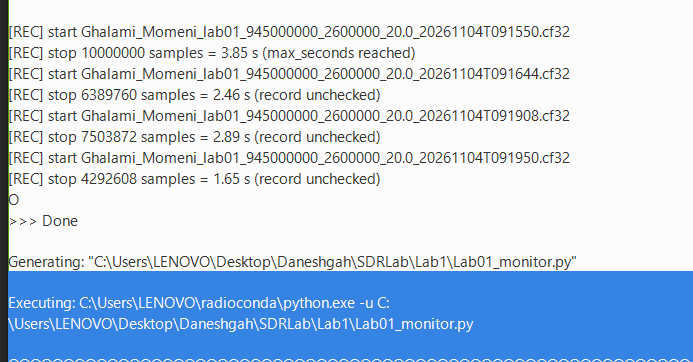
\includegraphics[width=0.96\linewidth,height=0.29\textheight,keepaspectratio]{../assets/images/lab01/Screenshot 2026-11-04 093343.png}\caption{\rtl{پیام‌های شروع و پایان ضبط؛ حجم مورد انتظار از شمار نمونه‌ها محاسبه می‌شود.}}\label{fig:19}\end{figure}
\rp{جدول \ref{tab:uncertainty} اطلاعات این بخش را ثبت می‌کند.}
\begin{table}[H]\centering\small\renewcommand{\arraystretch}{1.25}
\begin{tabular}{|p{0.445\linewidth}|p{0.445\linewidth}|}\hline
\rtl{\textbf{کمّی‌سازی}} & \rtl{\textbf{منبع}} \\ \hline
\rtl{در \lr{2.6 MS/s: Δf=2.5390625 kHz}؛ در \lr{20 MS/s: Δf=19.53125 kHz}} & \rtl{تفکیک \lr{FFT} با \lr{N=1024}} \\ \hline
\rtl{اگر فقط نزدیک‌ترین خانه خوانده شود: حدود \lr{±Δf/2}؛ پنجره، \lr{SNR} و بایاس نیز مؤثرند} & \rtl{کوانتیزهٔ انتخاب خانهٔ قله} \\ \hline
\rtl{حد بدبینانه از خطای خانه‌ها حدود \lr{±Δf}؛ دقت واقعی به شیب لبه و کف نویز هم وابسته است} & \rtl{خطای پهنا از دو لبه} \\ \hline
\rtl{در \lr{434 MHz: ±10.85 kHz}؛ در \lr{945 MHz: ±23.625 kHz}؛ مشخصهٔ قطعی دستگاه فعلی نیست} & \rtl{مرجع فرضی \lr{±25 ppm}} \\ \hline
\rtl{حدود \lr{±0.2 MHz} یا بیشتر؛ برای \lr{B99}، \lr{B6/B20} یا \lr{ppm} کافی نیست} & \rtl{خوانش بلوک‌ها از تصویر} \\ \hline
\rtl{۸ بایت/نمونه؛ \lr{2.6 MS/s} یعنی \lr{20.8 MB/s} و \lr{20 MS/s} یعنی \lr{160 MB/s}؛ نرخ فایل مدت دیواری را تضمین نمی‌کند} & \rtl{انتقال فایل \lr{cf32}} \\ \hline
\end{tabular}\caption{\rtl{مقیاس‌های خطا؛ این مقادیر حد تضمین‌شدهٔ کل اندازه‌گیری نیستند}}\label{tab:uncertainty}\end{table}
\rp{پردازش تحویلی از \lr{cf32} با ترتیب \lr{I,Q} و \lr{little-endian} استفاده می‌کند، میانگین \lr{Welch} را در مقیاس خطی و با پنجرهٔ \lr{Hann} می‌سازد و پس از آن به \lr{dB} تبدیل می‌کند. برای هر سیگنال باید بازهٔ جداگانهٔ \lr{RF} انتخاب شود؛ انتگرال‌گیری روی کل باند چندحاملی پهنای یک سیگنال نیست. \lr{B99} از صدک‌های تجمعی ۰٫۵٪ و ۹۹٫۵٪ در همان بازه به دست می‌آید؛ نتیجه با کف نویز موجود محاسبه می‌شود و وابستگی آن به \lr{ROI} در خروجی ثبت می‌شود. سطح \lr{PSD} با واحد توان نسبی بر \lr{Hz} است؛ بدون کالیبراسیون، \lr{dBm} نیست و در صورت نامعلوم‌بودن مقیاس نمونه‌ها، \lr{dBFS} نامیده نمی‌شود.}

\rp{آبشار آفلاین از تمام نمونه‌ها در قاب‌های پی‌درپی ساخته می‌شود؛ برای تصویر نهایی قاب‌ها گروه‌بندی می‌شوند و حداقل/حداکثر زمان هر گروه حفظ می‌شود. یک فایل فاقد \lr{timestamp} یا شمارندهٔ سخت‌افزار نمی‌تواند نبود نمونه‌های ازدست‌رفته در شبکه را ثابت کند. اندازه‌گیری برست با مسیر جداگانهٔ توان کانال و گام زمانی ۰٫۱ \lr{ms} انجام می‌شود؛ آستانه باید از قطعهٔ خاموش انتخاب و حساسیت نتیجه به آن بررسی شود. حذف گذرای فیلتر در ابتدای فایل و علامت‌زدن رویداد بریده در انتها ضروری است.}

\rp{کد موجود تنها پس از معرفی فایل، \lr{fs}، مرکز واقعی و \lr{ROI} اجرا می‌شود. خروجی ساختگی به سایت تزریق نشده است. پس از تحلیل، \lr{tools/lab01\_publish\_analysis.py} جدول‌ها و نمودارهای واقعی را به بخش جداگانهٔ گزارش اضافه می‌کند؛ تکمیل تشخیص فناوری، \lr{ppm} و تطبیق پرسش‌ها همچنان نیازمند بازبینی علمی گروه است.}

\Needspace{6\baselineskip}
\section{\rtl{۸. عیب‌یابی و کارهایی که بار بعد تغییر می‌دهیم}}
\rp{خطای نصب یا قطع اتصال از تصاویر اثبات نشده است؛ \lr{ping} موفق است. مسائل مستند تحلیل عبارت‌اند از نام‌گذاری گمراه‌کنندهٔ \lr{radio}، تغییر محور در \lr{DCoff}، \lr{lo\_shift} غیرصفر در بخشی از ثبت‌ها و نبود دفتر شمارش برست‌ها. پیام‌های \lr{U/O} یا نویسه‌های تکراری کنسول به‌تنهایی مقدار افت داده را تعیین نمی‌کنند و باید همراه با نسخهٔ نرم‌افزار و شمارنده‌های انتقال تفسیر شوند.}

\begin{itemize}
\item \rtl{همراه هر ضبط، \lr{RX LO} و \lr{TX LO}، نرخ واقعی، بهره، تضعیف، حالت \lr{DC/IQ}، اتصال، پنجره، \lr{FFT} و زمان شروع را در \lr{JSON} ثبت می‌کنیم؛ پس از هر تغییر حافظهٔ \lr{Max Hold} را پاک می‌کنیم.}
\item \rtl{برای پهنای چندمگاهرتزی نرخ کافی و برای زمان‌بندی برست نرخ \lr{2.6 MS/s} با کنترل افت نمونه انتخاب می‌کنیم؛ ضبط باریک جای نمای کامل سیگنال پهن را نمی‌گیرد.}
\item \rtl{در آزمون \lr{LO}، یک جدول هم‌زمان برای همهٔ قله‌ها و حداقل سه مقدار شیفت ثبت می‌کنیم؛ \lr{DC} روشن/خاموش را با تنظیم و اتصال یکسان می‌سنجیم.}
\item \rtl{تعداد فشردن ریموت و زمان هرکدام را با شمارنده ثبت می‌کنیم و کلیپ صوتی/ویدئو را جای ساعت نمونهٔ \lr{IQ} نمی‌گیریم.}
\item \rtl{برای آزمون اشباع، بهره را ۵ تا ۱۰ \lr{dB} کم می‌کنیم و تغییر نسبی قله‌های اصلی و جانبی و دامنهٔ نمونه‌ها را مقایسه می‌کنیم.}
\end{itemize}
\Needspace{6\baselineskip}
\section{\rtl{۹. وضعیت تکمیل الزامات}}
\rp{جدول \ref{tab:completion} اطلاعات این بخش را ثبت می‌کند.}
\begin{table}[H]\centering\small\renewcommand{\arraystretch}{1.25}
\begin{tabular}{|p{0.445\linewidth}|p{0.445\linewidth}|}\hline
\rtl{\textbf{وضعیت}} & \rtl{\textbf{الزام}} \\ \hline
\rtl{پاسخ مفهومی کامل؛ نتایج تجربی سؤال ۲، بخشی از ۴ و شمارش سؤال ۷ در انتظار داده} & \rtl{پاسخ پرسش‌های ۱ تا ۸} \\ \hline
\rtl{پنج نامزد معرفی شده؛ اندازه‌گیری مستقل و انتساب فایل‌ها لازم است} & \rtl{پنج سیگنال در سه محدوده} \\ \hline
\rtl{کد آماده؛ داده و نمودار تجربی هنوز موجود نیست} & \rtl{\lr{Welch} و \lr{OBW99} از \lr{IQ}} \\ \hline
\rtl{کد آماده؛ اجرای دادهٔ ریموت پیوسته و آستانهٔ معتبر لازم است} & \rtl{آبشار و زمان برست} \\ \hline
\rtl{کد آماده؛ فایل حلقه و \lr{f\_tx} واقعی لازم است} & \rtl{برآورد دقیق تن حلقه} \\ \hline
\rtl{نیازمند حامل \lr{GSM} تأییدشده و ثبت مرکز و پیوستگی} & \rtl{\lr{ppm} و دو کانال \lr{BCCH}} \\ \hline
\rtl{نسخهٔ قبلی در \lr{reports/lab01-prelab} موجود؛ یکسان‌بودن با اجرای جلسه نیازمند تأیید} & \rtl{فلوگراف و ضبط‌کننده} \\ \hline
\rtl{لاگ بازسازی‌شده از تصاویر ارائه شده؛ تقسیم کار و ساعت دستگاه نیازمند تکمیل} & \rtl{لاگ و نقش اعضا} \\ \hline
\end{tabular}\caption{\rtl{تحویل علمی پس از دریافت فایل‌های هم‌گروهی تکمیل می‌شود}}\label{tab:completion}\end{table}
\Needspace{6\baselineskip}
\section{\rtl{۱۰. فایل‌ها و اجرای تحلیل}}
\rp{نسخهٔ HTML همین گزارش، PDF، منبع LaTeX، مراجع BibTeX و فایل‌های همراه از صفحهٔ گزارش در وب‌سایت قابل دریافت‌اند. در آرشیو نیمسال، پیش‌گزارش و گزارش هر آزمایش مسیرهای مستقلی دارند.}

\rp{راهنمای \lr{LAB01-UPDATE.md} در ریشهٔ مخزن، مراحل افزودن \lr{IQ} و بازسازی سایت را توضیح می‌دهد. همهٔ تصاویر با نام اصلی در \lr{assets/images/lab01} و فهرست قابل تطبیق در \lr{evidence-manifest.json} نگهداری شده‌اند.}

\clearpage
\Needspace{6\baselineskip}
\section{\rtl{مراجع}}
\rp{[۱] دستور کار آزمایش ۱: پایش طیف، \lr{lab\_01\_spectrum\_final (2).pdf}، ۱۹ صفحه؛ پرسش‌ها در صفحات ۹-۱۵، الزامات تحلیل در صفحهٔ ۱۵.}

\rp{[۲] \lr{photos.zip}، شامل ۳۷ تصویر اصلی ثبت‌شدهٔ گروه؛ اعداد مشاهده‌ای با نام تصویر در متن مشخص شده‌اند.}

\rp{[۳] \lr{ETSI TS 136 104 V18.5.0}، جدول \lr{5.6-1:} پهنای کانال و تعداد \lr{RB.} }

\begin{flushleft}\small\url{https://www.etsi.org/deliver/etsi_TS/136100_136199/136104/18.05.00_60/ts_136104v180500p.pdf}\end{flushleft}
\rp{[۴] \lr{ETSI TS 125 104 V3.8.0}، بخش‌های ۵٫۱ و ۵٫۴٫۱: نرخ تراشه و فاصلهٔ کانال \lr{UTRA FDD.} }

\begin{flushleft}\small\url{https://www.etsi.org/deliver/etsi_ts/125100_125199/125104/03.08.00_60/ts_125104v030800p.pdf}\end{flushleft}
\rp{[۵] \lr{ETSI TS 136 211 V15.8.1}، ساختار نماد \lr{OFDM} و \lr{CP.} }

\begin{flushleft}\small\url{https://www.etsi.org/deliver/etsi_ts/136200_136299/136211/15.08.01_60/ts_136211v150801p.pdf}\end{flushleft}
\end{document}
